\documentclass[11pt, mathserif, handout, table]{beamer}

% ================== PACKAGES ==================
\usepackage{amsmath}
\usepackage{amssymb}
\usepackage{amsthm}
\usepackage{array}
\usepackage{bbm}
\usepackage{caption}
\usepackage{color}
\usepackage{fancyvrb}
\usepackage[T1]{fontenc}
% \usepackage[pdftex]{graphicx}
% \usepackage{handoutWithNotes}
\usepackage{hyperref}
\usepackage{multirow}
\usepackage{nicefrac}
\usepackage{subcaption}
\usepackage{tikz}
\usepackage{qtree}
\usepackage{wrapfig}
\usepackage{xcolor}
\usetikzlibrary{arrows,shapes}

%%%%%%%%%%%%%%%%%%%%%%%%%%%%% Useful math macros %%%%%%%%%%%%%%%%%%%%%%%%%%%%%%%
% argmax and argmin
\DeclareMathOperator*{\argmax}{arg\,max}
\DeclareMathOperator*{\argmin}{arg\,min}

%% Distributions
\newcommand{\Norm}[2]{\mathcal{N}(#1,#2)}
\newcommand{\Unif}{\mathsf{U}}
\newcommand{\Pois}[1]{\mathsf{Poisson}(#1)}
\newcommand{\Exp}[1]{\mathsf{Exponential}(#1)}
\newcommand{\Gamm}[2]{\mathsf{Gamma}(#1,#2)}
\newcommand{\Bern}[1]{\mathsf{Bernoulli}\left(#1\right)}
\newcommand{\Binom}[2]{\mathsf{Binom}(#1,#2)}
\newcommand{\Geom}[1]{\mathsf{Geometric}(#1)}
\newcommand{\Cat}{\mathsf{Categorical}}
\newcommand{\Beta}[2]{\mathsf{Beta}(#1,#2)}
\newcommand{\Lapl}{\mathsf{Laplace}}
\newcommand{\GP}{\mathcal{GP}}
\newcommand{\DP}[1]{\mathsf{DP}(#1)}
\newcommand{\CRP}[1]{\mathsf{CRP}(#1)}
\newcommand{\GEM}[1]{\mathsf{GEM}(#1)}
\newcommand{\Dir}[1]{\mathsf{Dirichlet}(#1)}
\newcommand{\Discrete}[1]{\mathsf{Discrete}(#1)}

%% Probability
\newcommand{\E}[1]{\mathbb{E}[#1]}
\newcommand{\V}[1]{\mathbb{V}[#1]}
\newcommand{\Cov}[2]{\mathbb{C}\mathrm{ov}(#1,#2)}
\newcommand{\given}{\, \vert \,}

%% General
\newcommand{\R}{\mathbb{R}}
\newcommand{\Z}{\mathbb{Z}}
\newcommand{\N}{\mathbb{N}}
\newcommand{\abs}[1]{\left\vert #1 \right\vert}
\newcommand{\norm}[1]{\left\vert \left \vert #1 \right\vert \right\vert}

%% Vectors and Matrices
\newcommand{\bx}{\mathbf{x}}
\newcommand{\bX}{\mathbf{X}}
\newcommand{\by}{\mathbf{y}}
\newcommand{\bY}{\mathbf{Y}}
\newcommand{\ba}{\mathbf{a}}
\newcommand{\bA}{\mathbf{A}}
\newcommand{\bb}{\mathbf{b}}
\newcommand{\bB}{\mathbf{B}}
\newcommand{\bc}{\mathbf{c}}
\newcommand{\bM}{\mathbf{M}}
\newcommand{\bC}{\mathbf{C}}
\newcommand{\bQ}{\mathbf{Q}}
\newcommand{\bl}{\mathbf{l}}
\newcommand{\bem}{\mathbf{m}}
\newcommand{\bq}{\mathbf{q}}
\newcommand{\bz}{\mathbf{z}}
\newcommand{\bZ}{\mathbf{Z}}
\newcommand{\bu}{\mathbf{u}}
\newcommand{\br}{\mathbf{r}}
\newcommand{\bs}{\mathbf{s}}
\newcommand{\bw}{\mathbf{w}}
\newcommand{\bW}{\mathbf{W}}
\newcommand{\bT}{\mathbf{T}}
\newcommand{\bth}{\bm\uptheta}
\newcommand{\bTh}{\bm\Theta}
\newcommand{\bbeta}{\boldsymbol{\beta}}
\newcommand{\btheta}{\boldsymbol{\theta}}
\newcommand{\bpi}{\boldsymbol{\pi}}
\newcommand{\bphi}{\boldsymbol{\phi}}
\newcommand{\btau}{\boldsymbol{\tau}}
\newcommand{\bmu}{\boldsymbol{\mu}}
\newcommand{\blambda}{\boldsymbol{\lambda}}
\newcommand{\bSigma}{\boldsymbol{\Sigma}}

%% Sets
\newcommand{\cA}{\mathcal{A}}
\newcommand{\cB}{\mathcal{B}}
\newcommand{\cZ}{\mathcal{Z}}
\newcommand{\cM}{\mathcal{M}}
% \usepackage{mathpazo}

% \mode<handout>{
% \pgfpagesuselayout{3 on 1 with notes}[letterpaper, border, shrink=0mm]
% }

\definecolor{paperbg}{HTML}{FDF6E3}
\definecolor{paperbgdark}{HTML}{EDE6CA}
\definecolor{solarred}{HTML}{DC322F}
\definecolor{solarlightorange}{HTML}{EBD6C3}
\definecolor{solarlightgreen}{HTML}{F3FFC8}
\definecolor{solarorange}{HTML}{C45B2A}
\definecolor{solaryellow}{HTML}{A57900}
\definecolor{solargreen}{HTML}{859900}
\definecolor{solarcyan}{HTML}{2AA198}
\definecolor{solarblue}{HTML}{268BD2}
\definecolor{solardarkblue}{HTML}{005BA2}
\definecolor{solarviolet}{HTML}{6C71C4}
\definecolor{solarmagenta}{HTML}{C05068}
\definecolor{solarbase2}{HTML}{EEE8D5}
\definecolor{solarbase1}{HTML}{93A1A1}
\definecolor{solarbase00}{HTML}{657B83}
\definecolor{solarbase01}{HTML}{586E75}
\definecolor{solarbase015}{HTML}{174652}
\definecolor{solarbase02}{HTML}{073642}
\definecolor{solarbase03}{HTML}{002B36}
\definecolor{functionblue}{HTML}{40A0B8}
\definecolor{solarlightblue}{HTML}{D9EEEF}

% \usetheme{Dresden}

\setbeamercolor{background canvas}{bg=paperbg}
% \mode<handout>{
% \setbeamercolor{background canvas}{bg=white}
% }
\setbeamercolor{normal text}{fg=solarbase01}
\usecolortheme[named=functionblue]{structure}
\setbeamercolor{title in sidebar}{fg=solaryellow}
\setbeamercolor{author in sidebar}{fg=solaryellow}
\setbeamercolor{section in head/foot}{fg=paperbg}
\setbeamercolor{section in sidebar}{fg=functionblue}
\setbeamercolor{section in sidebar shaded}{fg=solarbase1}

\usecolortheme{orchid}
\setbeamercolor{block body}{fg=solarbase01, bg=solarlightgreen}
\setbeamercolor{block title}{fg=paperbg, bg=solargreen}
\setbeamercolor{alertblock body}{fg=solarbase01, bg=solarlightorange}
\setbeamercolor{alertblock title}{fg=paperbg, bg=solarorange}
\setbeamertemplate{navigation symbols}{}

\newenvironment<>{attnblock}[1]{%
  \begin{actionenv}#2%  
      \def\insertblocktitle{#1}%
      \par%
      \mode<presentation>{%
        \setbeamercolor{block title}{fg=paperbg, bg=solarorange}
        \setbeamercolor{block body}{fg=solarbase01, bg=solarlightorange}
        \setbeamercolor{itemize item}{fg=solarorange}
        \setbeamercolor{itemize subitem}{fg=solarorange}
        }%
      \usebeamertemplate{block begin}}
{\par\usebeamertemplate{block end}\end{actionenv}}

\newenvironment<>{infoblock}[1]{%
  \begin{actionenv}#2%  
      \def\insertblocktitle{#1}%
      \par%
      \mode<presentation>{%
        \setbeamercolor{block title}{fg=paperbg, bg=solargreen}
        \setbeamercolor{block body}{fg=solarbase01, bg=solarlightgreen}
        \setbeamercolor{itemize item}{fg=solargreen}
        \setbeamercolor{itemize subitem}{fg=solargreen}
        \setbeamercolor{enumerate item}{fg=solargreen}
        }%
      \usebeamertemplate{block begin}}
{\par\usebeamertemplate{block end}\end{actionenv}}

\newenvironment<>{exblock}[1]{%
  \begin{actionenv}#2%  
      \def\insertblocktitle{#1}%
      \par%
      \mode<presentation>{%
        \setbeamercolor{block title}{fg=paperbg, bg=functionblue}
        \setbeamercolor{block body}{fg=solarbase01, bg=solarlightblue}
        \setbeamercolor{itemize item}{fg=functionblue}
        \setbeamercolor{itemize subitem}{fg=functionblue}
        }%
      \usebeamertemplate{block begin}}
{\par\usebeamertemplate{block end}\end{actionenv}}

% Double-line for start and end of epigraph.
\newcommand{\epiline}{\hrule \vskip -.2em \hrule}
% Massively humongous opening quotation mark.
\newcommand{\hugequote}{%
  \fontsize{42}{48}\selectfont \color{solarcyan} {\rm \textbf{``}}
  \vskip -.5em
}

% Beautify quotations.
\newcommand{\epigraph}[3]{%
  \bigskip
  \colorbox{solarbase2}{%
    \parbox{#1\textwidth}{%
    \epiline \vskip 1em {\hugequote} % \vskip -.5em
    % \parindent 2.2em
    {\rm #2}\begin{flushright}{\rm  #3}\end{flushright}
    \epiline
    }
  }
  \bigskip
}

\title{HaMMLeT: An Infinite-State Hidden Markov Model With Local Transitions}
\author{Colin Reimer Dawson}
\date{8 August 2016}

\begin{document}

\frame{\titlepage}

\begin{frame}
  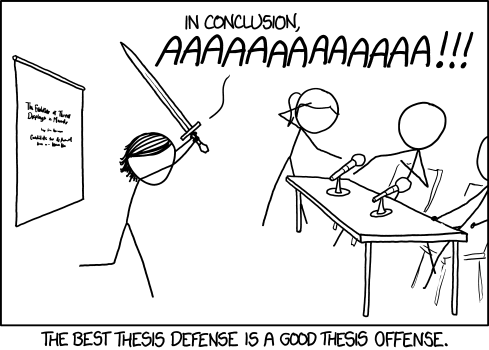
\includegraphics[width=\textwidth]{img/defense.png}
\end{frame}

\begin{frame}
  \frametitle{Outline}
  \tableofcontents
\end{frame}

% ====================================================

\section{Some Motivating Applications}
\begin{frame}
  \frametitle{Biological Context in Text}
  \begin{exampleblock}{\small
  \begin{quote}
    Mutations in oncogenes are much more likely to lead to cancer in
    some tissue types than others, because some tissues express other 
    proteins that counteract the oncogene.  For example, in {\color{solarred}{MICE}} the 
    {\color{solargreen}{G12D activating mutation in K-ras}} causes
    {\color{solarorange}{lung}} tumors but {\color{solarorange}{not 
    muscle-derived}} sarcomas, because muscle cells express two proteins 
    (Arf and Ink4a) that cause cell division to halt when Ras is
    overactive.        

    \vspace{0.2in}
    (Young and Jacks, PNAS, 2010)
  \end{quote}
}
\end{exampleblock}
\end{frame}

\begin{frame}{Biological Context in Text}
  \begin{center}
    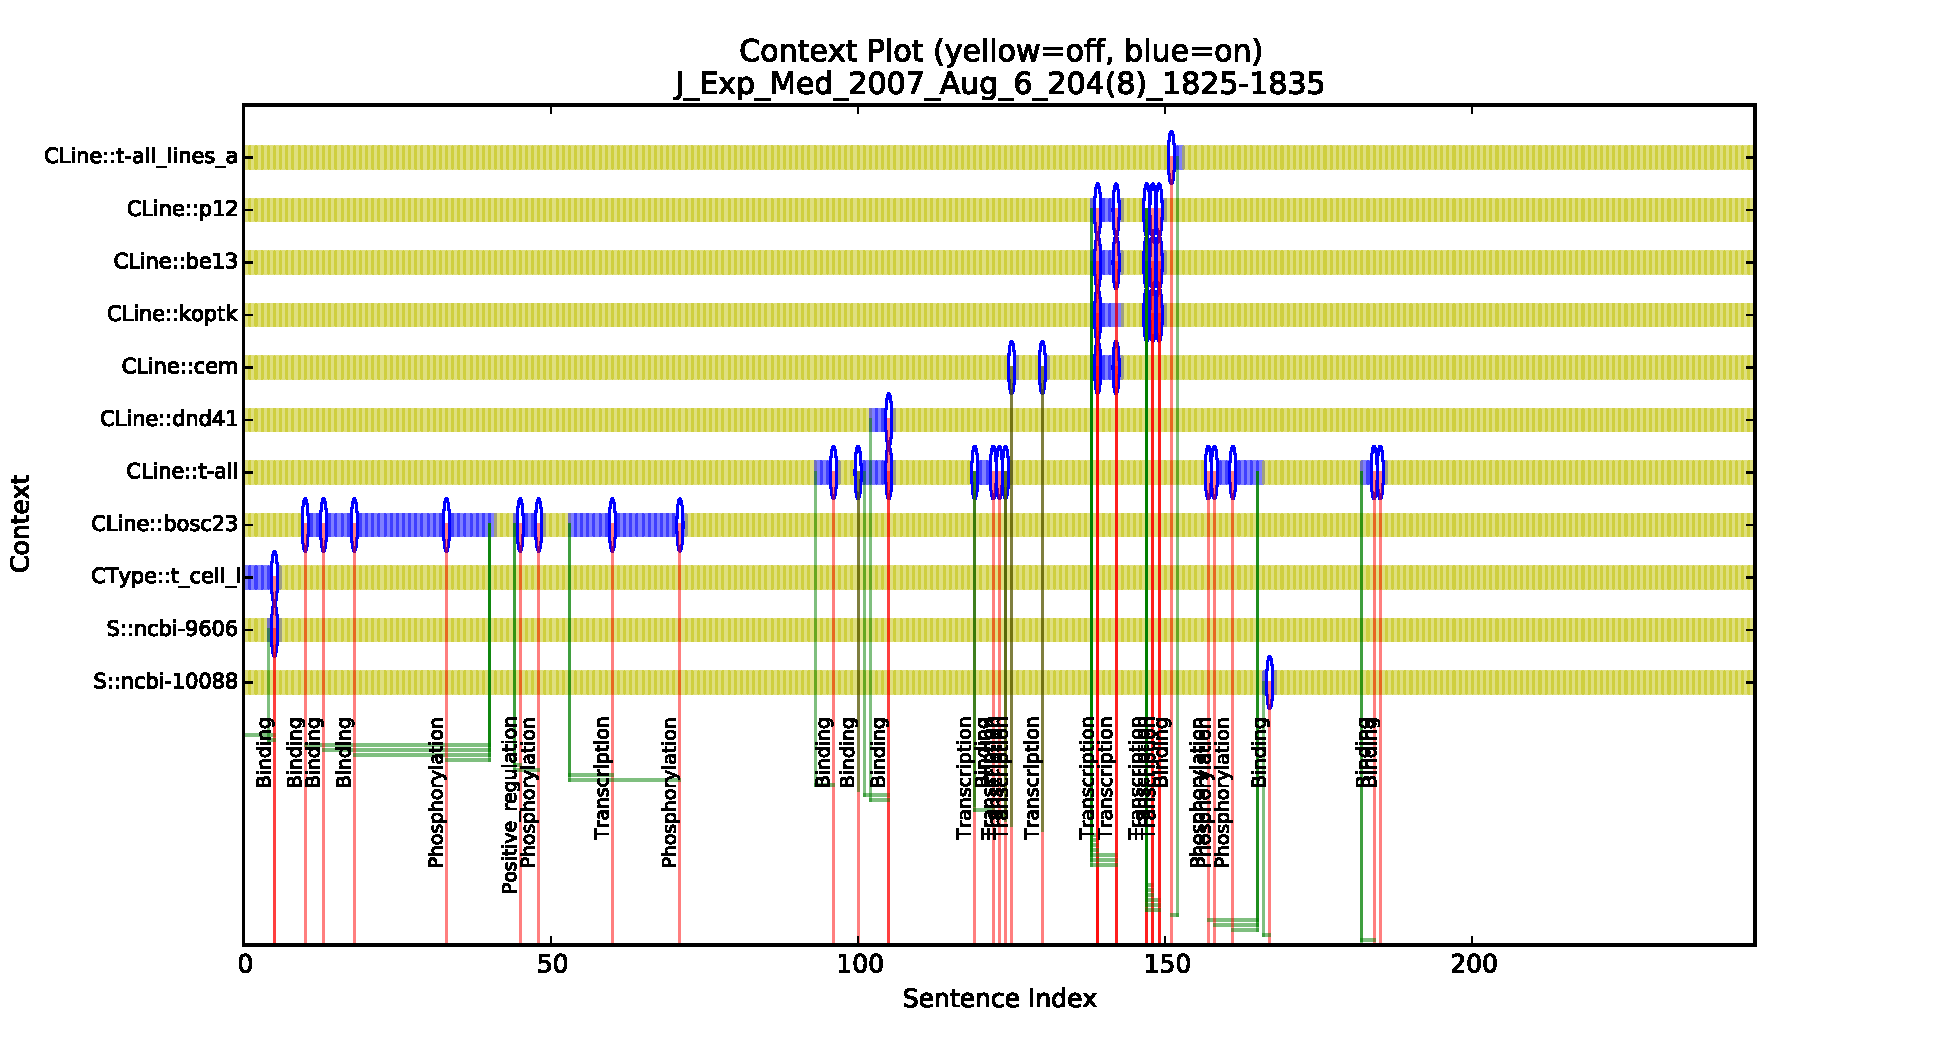
\includegraphics[width=\textwidth]{img/bio_contexts.pdf}
  \end{center}
\end{frame}

\begin{frame}{Blind Source Separation: The ``Cocktail Party'' Problem}
  \begin{center}
    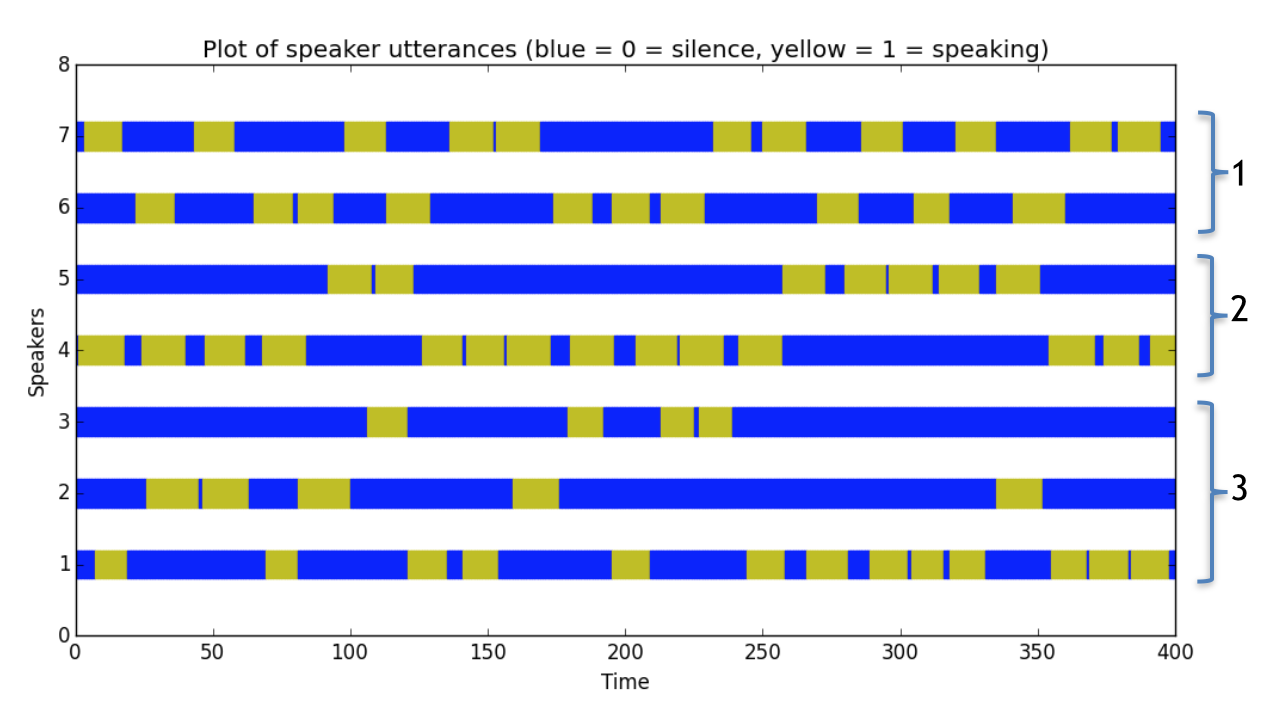
\includegraphics[width=\textwidth]{img/cocktail-with-groups.png}
  \end{center}
\end{frame}

\begin{frame}
  \frametitle{Cocktail Party Data}
\href{http://research.ics.aalto.fi/ica/cocktail/011001010mix1.wav}{{\color{solarmagenta}{A
  ``Cocktail Party''}}}
\end{frame}

% \begin{frame}
%   \frametitle{Markov Chains}
%   \begin{center}
%     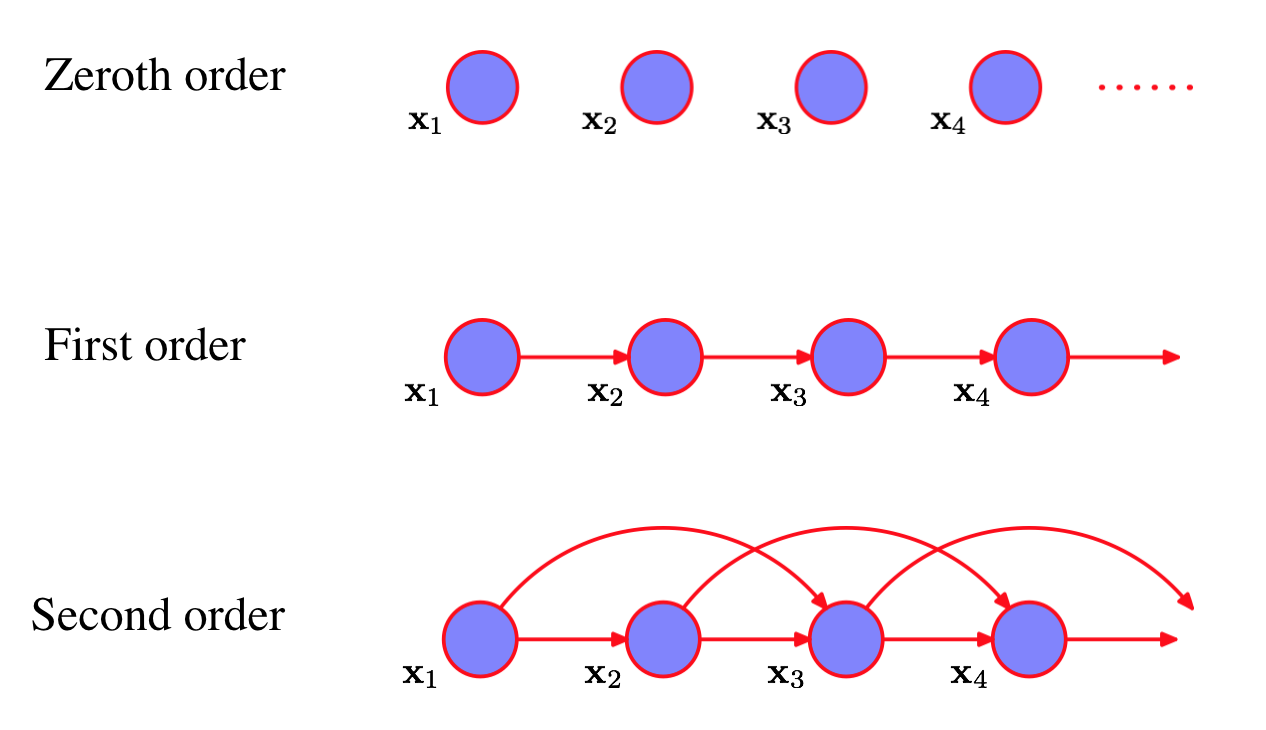
\includegraphics[width=\textwidth]{img/markov_bishop.png}
%   \end{center}

% \begin{exampleblock}{\small
% Note: The directed graph representation of the factorization of a
% joint distribution is called a {\bf Bayes' Net}
% }
% \end{exampleblock}
% \end{frame}

% \begin{frame}{Example Markov Chain}
%   \begin{center}
%     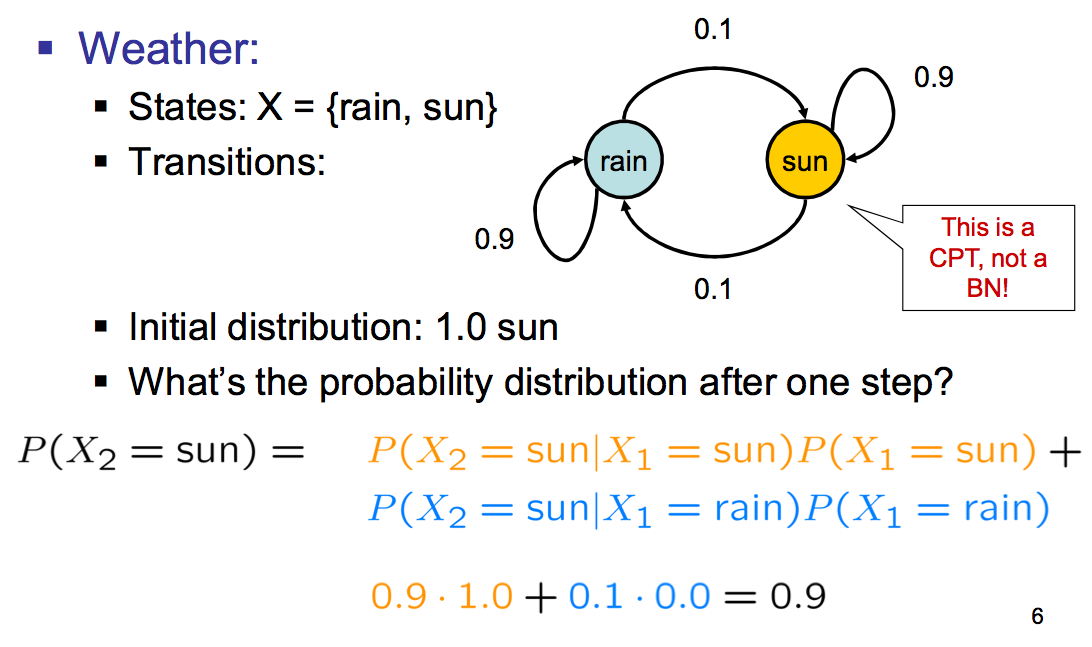
\includegraphics[width=\textwidth]{img/Weather_chain.png}
%   \end{center}
% \end{frame}

\section{Hidden Markov Models (HMMs)}

\begin{frame}{Hidden Markov Model}
Data depends at each $t$ on an {\em unobserved} state, $z_t$, which
evolve as a Markov chain.
\begin{center}
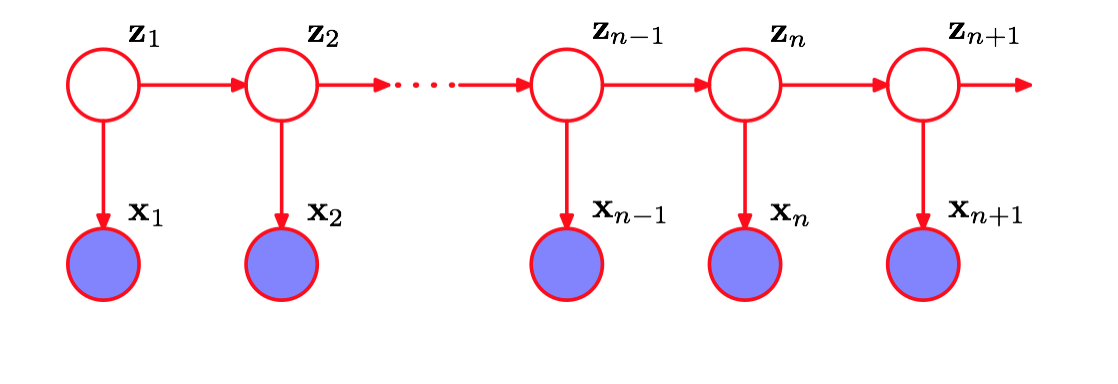
\includegraphics[width=\textwidth]{img/hmm_bishop.png}
\end{center}
\end{frame}

\begin{frame}{HMM Example}
\begin{center}
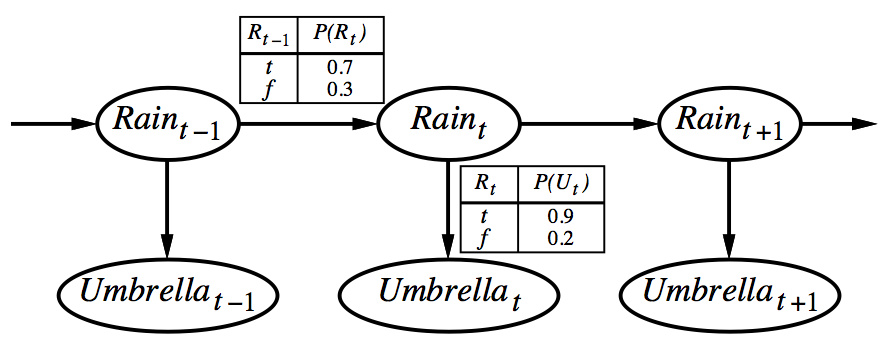
\includegraphics[width=\textwidth]{img/hmm_umbrella.png}
\end{center}

\begin{center}
\begin{minipage}{0.5\textwidth}
\begin{exampleblock}{\small
 The HMM is defined by:

\begin{tabular}{ll}
Initial distribution & $\pi_0$\\
Transition matrix & $\pi$ \\
Emission distributions & $\{F_k\}$
\end{tabular}
}
\end{exampleblock}
\end{minipage}
\end{center}
\end{frame}

% \begin{frame}{Hidden Markov Model}
% \begin{exampleblock}{\small
%     Let $\{F_k\}_{k=1}^K$ be a family of distributions on $\mathcal{X}$ and
%     $(\pi)_{kk'}$ a $K\times K$ {\bf transition matrix} (with $\pi_k$ the
%     $k$th row), and $\pi_0$ an {\bf initial distribution}.  Define a {\bf latent state
%       sequence}, $\{z_t\}_{t=1}^T$ and an {\bf observation sequence}
%     $\{x_t\}_{t=1}^T$ such that
%     \begin{align}
%       \label{eq:12}
%       z_t \given z_{t-1} &\sim \pi_{z_{t-1}} \quad t = 1, \dots, T \\
%       x_t \given z_t &\sim F_{z_t} \qquad t = 1, \dots, T
%     \end{align}
%     with $z_0 := 0$.  This defines a {\bf Hidden Markov
%       Model} (HMM).
% }
% \end{exampleblock}
% \end{frame}

\begin{frame}{Applications of HMMs}
  Speech recognition
  \begin{itemize}
  \item $Y_t$: acoustic signal
  \item $Z_t$: word segments
  \end{itemize}
  Machine translation
  \begin{itemize}
  \item $Y_t$: words in language A
  \item $Z_t$: words in language B
  \end{itemize}
  Robot tracking
  \begin{itemize}
  \item $Y_t$: sensor data
  \item $Z_t$: real position in space
  \end{itemize}
\end{frame}

\begin{frame}{Some Inference Objectives for HMMs}
  \begin{enumerate}
  \item Given data, find good parameters
    (estimation)
  \item Given parameters and data, find the distribution over states at a
    particular $t$ (marginalization).
  \item Given parameters and data, find the most likely joint state
    sequence (maximization).
  \end{enumerate}
  
\end{frame}

\subsection{Mixture Models}
\label{sec:mixture-models}

\begin{frame}{HMMs as Mixture Models}
  HMMs can be viewed as a dynamic version of a {\bf mixture model}
  \begin{itemize}[<+->]
  \item Each data point, $y \in \mathcal{Y}$, 
    arises from one of several {\em classes}, each with its
    own distribution.
  \item Goal: Estimate unknown density, $f$, of the form
    \begin{equation*}
      \label{eq:3}
      f(y) = \sum_{j} \pi_j f_k(y)
    \end{equation*}
  \item Traditionally, number of components is fixed and $f_k$ have parametric form:
    \begin{equation}
      \label{eq:4}
      f(y; \pi, \theta) = \sum_{k=1}^K \pi_k f(y; \theta_k)
    \end{equation}
  \item Goal reduces to estimating $\pi$ and $\theta$.
  \end{itemize}
\end{frame}

\begin{frame}{Data from a Mixture Model}
  \begin{center}
    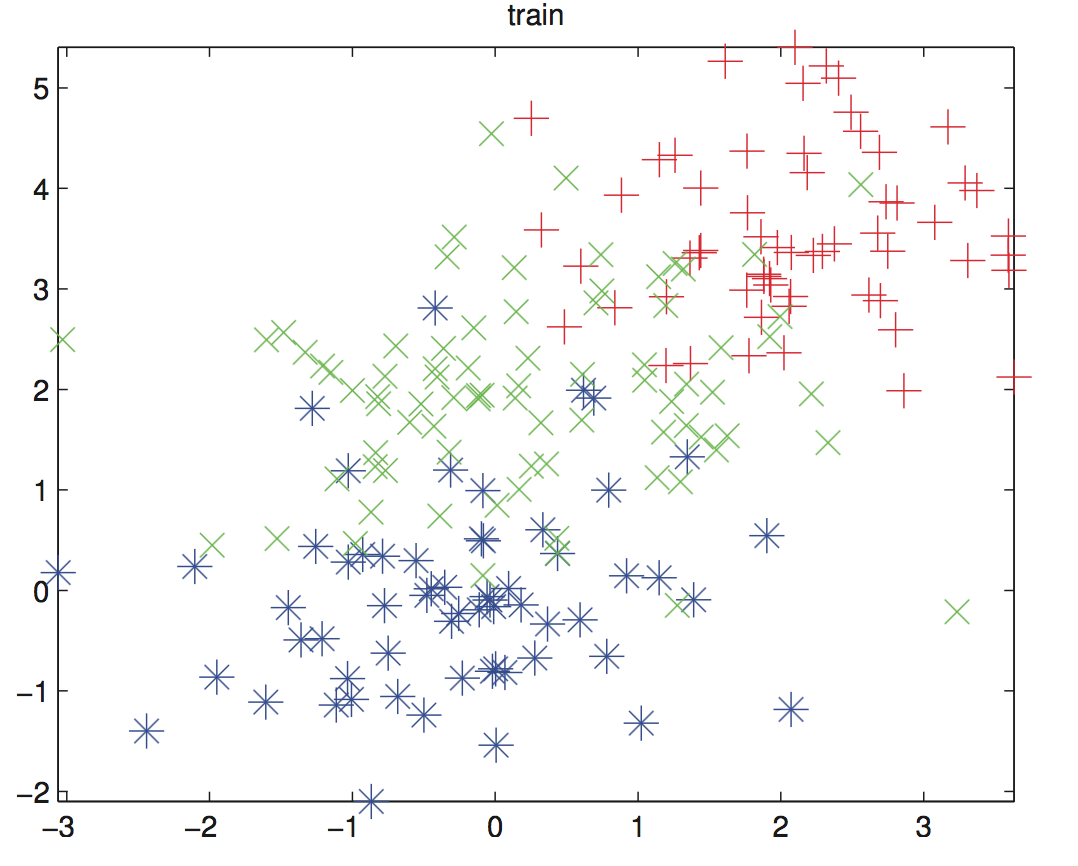
\includegraphics[width=0.8\textwidth]{img/knn_data.png}
  \end{center}
\end{frame}

\begin{frame}{A Mixture Density}
  \begin{center}
    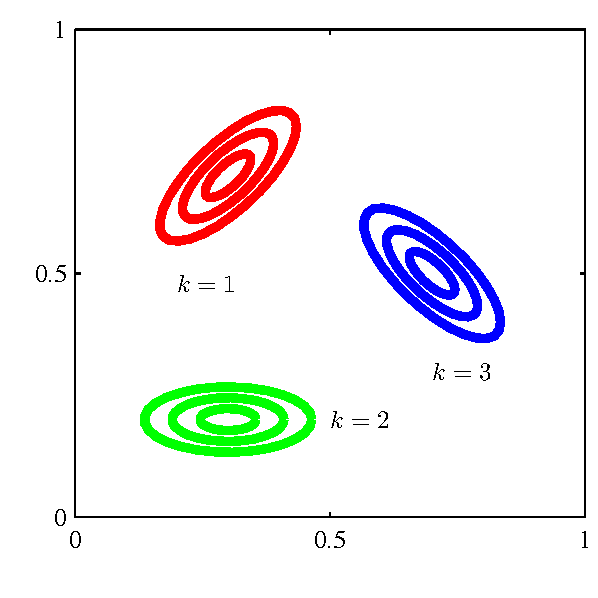
\includegraphics[width=0.8\textwidth]{img/mixture_density.pdf}
  \end{center}
\end{frame}
% ---------------------------------------------------

\begin{frame}
  \frametitle{A Bayesian Approach to Mixture Models}
% \begin{center}
% \colorbox{solarbase2}{
%   \begin{tabular}{ll}
%     \color{solarorange}{$f(\theta, \pi)$} & \color{solarorange}{Prior
%       density of $\theta, \pi$} \\
%     \color{solarblue}{$f(y|\theta,\pi)$} & \color{solarblue}{Likelihood
%       function $\theta,\pi$?}
%     \\
%     \color{solargreen}{$f(x)$} & \color{solargreen}{Average
%       likelihood of $x$ under all $\pi,\theta$}\\
%     \color{solarviolet}{$f(\pi,\theta \given x)$} &
%     \color{solarviolet}{Plausibility of $\pi$,$\theta$ after seeing
%       some data}
%   \end{tabular}
% }
% \end{center}
\begin{align*}
  {\color{solarviolet}{f(\theta, \pi \given x)}} &=
  {\color{solarorange}{f(\theta,\pi)}} \frac{\color{solarblue}{f(x \given
      \theta, \pi)}}{\color{solargreen}{f(x)}}\\
  &\propto {\color{solarorange}{f(\theta,\pi)}} {\color{solarblue}{f(x \given
      \theta, \pi)}}
\end{align*}
Standard Bayesian version uses {\em conjugate priors}: the family is
  closed under Bayesian updating (for a particular likelihood
  family).  {\bf Makes inference simple!}
\end{frame}

\begin{frame}{A Dynamic Mixture}
\begin{minipage}{0.45\textwidth}
    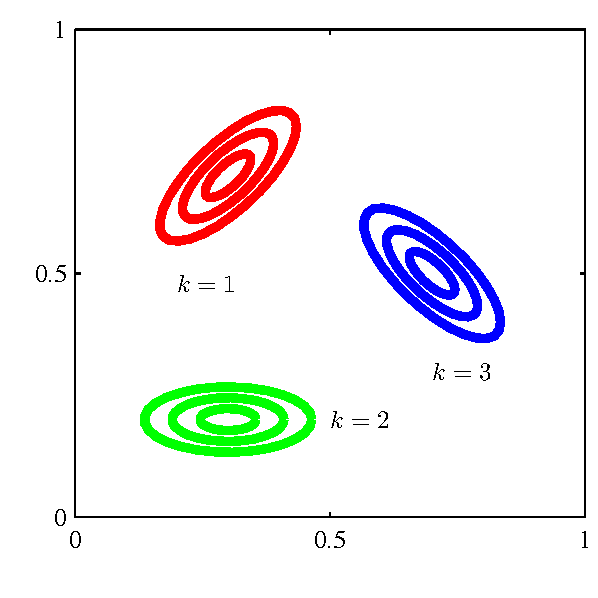
\includegraphics[width=\textwidth]{img/mixture_density.pdf}
  \end{minipage}
\hspace{0.1in}
\begin{minipage}{0.45\textwidth}
    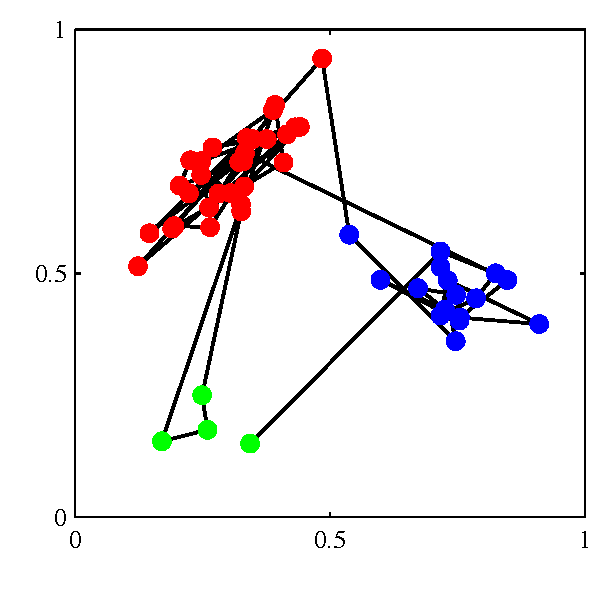
\includegraphics[width=\textwidth]{img/state_transitions.pdf}
  \end{minipage}
\end{frame}

% ---------------------------------------------------
\begin{frame}
  \frametitle{A Bayesian HMM}
An HMM allows the mixing weights to change depending on the previous
state.

\vspace{0.2in}
Standard: separate conjugate (Dirichlet) priors for each transition row $\pi_k$
\begin{minipage}{0.45\textwidth}
\begin{align*}
  \label{eq:5}
  \pi_k &\stackrel{i.i.d}{\sim} \mathrm{Dirichlet}(\alpha\mathbf{1}_K) \\
  \theta_k &\stackrel{i.i.d.}{\sim} f\text{-}\mathrm{Conjugate}(\xi)
\end{align*}
\end{minipage}
\hspace{0.1in}
\begin{minipage}{0.45\textwidth}
\begin{center}
  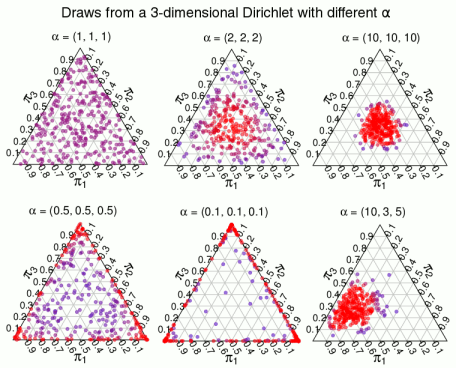
\includegraphics[width=\textwidth]{img/dirichlet.png}
\end{center}
\end{minipage}
\end{frame}
% ---------------------------------------------------
\section{``Nonparametric'' Bayesian Models}
\subsection{Infinite Mixture Models}
\label{sec:dirichl-proc-mixt}
\begin{frame}
  \frametitle{Unbounded number of components}
  \begin{itemize}[<+->]
  \item Having to specify $K$ in advance is limiting.  Too high $\to$
    overfitting.  Too low $\to$ underfitting.
  \begin{minipage}{0.4\textwidth}
    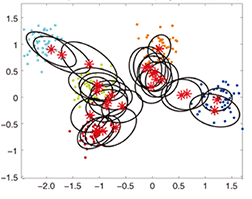
\includegraphics[width=\textwidth]{img/overfitting.png}
  \end{minipage}
  \hspace{0.1in}
  \begin{minipage}{0.4\textwidth}
    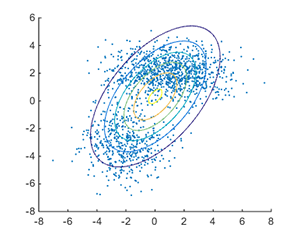
\includegraphics[width=\textwidth]{img/underfitting.png}
  \end{minipage}
  \item We can instead use an {\it infinite mixture model}, with a
    prior to guard against overfitting.
  \end{itemize}
\end{frame}

\begin{frame}
  \frametitle{Dirichlet Processes}
  \begin{exampleblock}{\small
      {\bf Definition: Dirichlet Process (Ferguson, 1973)}

\vspace{0.1in}
    A {\bf Dirichlet Process} with {\bf
      base probability measure} $G_0$ and {\bf concentration
      parameter} $\alpha > 0$ is a random measure, $\mu$ on a measure
    space $(\cX, \Sigma)$ with the property that, for any finite
    partition, $\{A_1, \dots, A_n\}$ of $\cX$,
    \begin{equation}
      \label{eq:6}
      (\mu(A_1), \dots, \mu(A_n)) \sim
      \mathrm{Dirichlet}(\alpha G_0(A_1), \dots, \alpha G_0(A_n))
    \end{equation}
}
  \end{exampleblock}

  \begin{itemize}
  \item Note 1: $\mu$ is atomic $a.s.$.
  \item Note 2: If $G_0$ has finite support, $\mu$ is just a
    Dirichlet distribution over those atoms.
  \end{itemize}
\end{frame}

\begin{frame}
  \frametitle{A Constructive Definition of the DP}
  \begin{exampleblock}{\small
      {\bf The Stick-Breaking Construction (Sethuraman, 1991)}
\vspace{0.1in}
    Define 
    \begin{align*}
      \{\tilde{\pi}_k\}_{k=1}^{\infty} &\stackrel{i.i.d}{\sim} \Beta{1}{\alpha}
      \\
      \pi_k &= \tilde{\pi}_k \prod_{k=1}^{k-1} (1 - \tilde{\pi_{k}}) \\
      \{\theta_k\}_{k=1}^{\infty} &\stackrel{i.i.d.}{\sim} G_0
    \end{align*}
    Then
      $\mu := \sum_{k=1}^{\infty} \pi_k \delta_{\theta_k}$
    is distributed $\mathsf{DP}(\alpha G_0)$
}
\end{exampleblock}
\vspace{-0.2in}
\begin{center}
  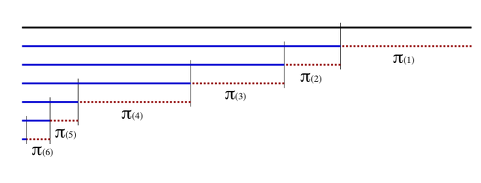
\includegraphics[width=1\textwidth]{img/stick-breaking.png}
\end{center}
\end{frame}

\begin{frame}
  \frametitle{An Infinite Mixture Model}
  \begin{exampleblock}{\small
      {\bf DP Mixture Model}
      \vspace{0.1in}

  If we let
  \begin{align}
    \label{eq:10}
    \pi &\sim \mathrm{Stick}(\alpha) \\
    \{\theta_k\} &\stackrel{i.i.d}{\sim} G_0 \\
    f(x \given \pi, \theta) &= \sum_{k=1}^\infty \pi_k f(x \given
    \theta_k)
  \end{align}
  then $x$ are distributed according to a {\bf Dirichlet Process
    Mixture Model}
}
\end{exampleblock}
\end{frame}

\begin{frame}{Infinite Gaussian Mixture Model}
For example, if $f(x \given \theta_k)$ is a Normal density, we
  have the {\bf Infinite Gaussian Mixture model} (Rasmussen, 2000)
  \begin{center}
    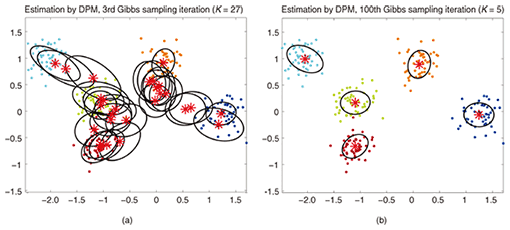
\includegraphics[width=\textwidth]{img/dp_clusters.png}
  \end{center}
\end{frame}

\subsection{An Infinite HMM?}
\label{sec:infinite-hmm}

\begin{frame}{Infinite State HMM}
  We want to allow HMM to have (countably) infinite state space.

\vspace{0.2in}
  Could put separate DP prior on each row of the transition matrix.
  Why might this not be ideal?

\pause

\vspace{0.2in}

{\color{solarorange}{We would never visit the same state twice!}}
\end{frame}

% ---------------------------------------------------
\subsection{Hierarchical Dirichlet Process Mixtures}
\label{sec:dirichl-proc-mixt}
\begin{frame}
  \frametitle{Hierarchical Dirichlet Processes}
  \begin{itemize}[<+->]
  \item Data from multiple sources, $j = 1, \dots, J$ (such
    as temporal contexts),
    whose generating distributions, $\{G_j\}$ are distinct but
    related.
\item Can use a hierarchical prior to couple them, e.g.,
    \begin{equation}
      \label{eq:11}
      G_j \stackrel{i.i.d}{\sim} \mathsf{DP}(\alpha G_0),
    \end{equation}
  \item But, if $G_0$ is absolutely continuous, sets of atoms in the
    $G_j$ will be disjoint.
  \item Solution: Let $G_0$ itself have a DP prior.
  \end{itemize}
\end{frame}

% ---------------------------------------------------
\begin{frame}
  \frametitle{Hierarchical Dirichlet Processes}
    \begin{exampleblock}{\small
        {\bf The Hierarchical Dirichlet Process Mixture Model (Teh,
          2006)}

\vspace{0.2in}
      Define
      \begin{align}
        G_0 &\sim \mathrm{DP}(\gamma H) \\
        G_j \given G_0 &\stackrel{i.i.d}{\sim} \mathrm{DP}(\alpha G_0)
        \qquad \qquad \quad j = 1, \dots, J\\
        y_{jn} \given G_j
        &\stackrel{i.i.d}{\sim} \sum_{k=1}^{\infty} \pi_{jk}
        f(\by \given \theta_{jk})
      \end{align}
      This defines a Hierarchical Dirichlet Process (HDP) Mixture.
      Atoms are shared among contexts by virtue of the discreteness of
      $G_0$.
}
    \end{exampleblock}
    \begin{itemize}
    \item $\gamma$: how close to ``uniform'' is the overall
      distribution of components?
    \item $\alpha$: how similar are the mixture weights across contexts?
    \end{itemize}
\end{frame}
% ---------------------------------------------------
\begin{frame}
  \frametitle{Examples of HDP Mixture Models}
  \begin{itemize}
  \item $f$ Normal: hierarchical Infinite Gaussian Mixture.
  \item $f$ Multinomial: {\bf hierarchical infinite topic model}
    \begin{itemize}
    \item $y$ words
    \item $\theta_{jk}$ word distributions corresponding to ``topics''
    \end{itemize}
  \end{itemize}
  \begin{center}
    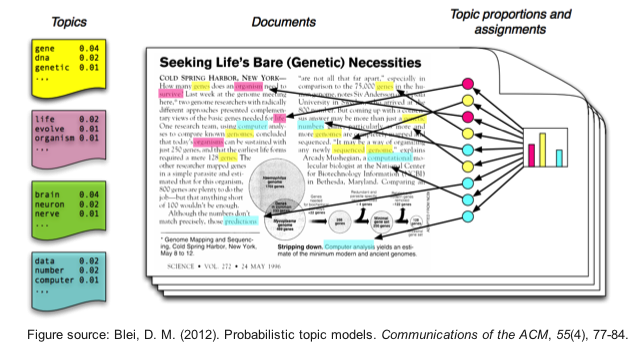
\includegraphics[width=\textwidth]{img/topic_models.png}
  \end{center}
\end{frame}
% ---------------------------------------------------


\begin{frame}

  \frametitle{An Infinite (HDP) HMM}
  We can allow infinitely many states by putting a Dirichlet Process
  prior on each row distribution, $\pi_j$.
  \begin{align}
    \label{eq:5}
    (\pi_j, \theta_j) &\stackrel{i.i.d}{\sim} \mathrm{DP}(\alpha G_0)
  \end{align}
  $\theta_j$: emission parameters for states
  reachable from state $j$.
  \pause

  \vspace{0.2in}

  To ensure that the $\theta_j$ contain overlapping values for 
  different $j$, $G_0$ must be discrete!
\pause
  \vspace{0.2in}
  Solution: A hierarchical prior: $G_0 \sim \mathrm{DP}(\gamma H)$.  
  This is the Infinite or HDP HMM (Beal, 2001; Teh, 2006).
\end{frame}

\begin{frame}{The HDP-HMM}
  \begin{center}
    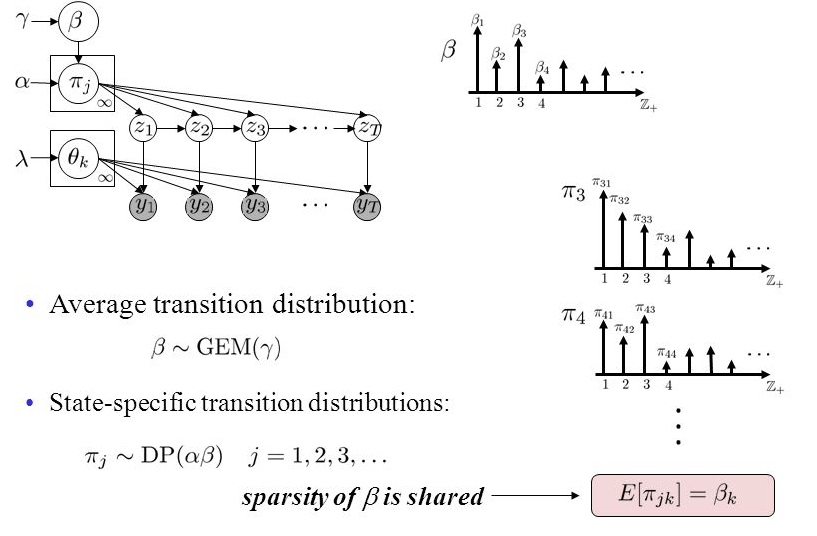
\includegraphics[width=\textwidth]{img/hdp_hmm.png}
  \end{center}
\end{frame}

\section{HDP HMM with Local Transitions}
\label{sec:hdp-hidden-markov}

%---------------------------------------------------
\subsection{Adding the Concept of ``Local'' Transitions}
\begin{frame}{Limitations of HDP-HMM}
  Two properties of HDP-HMM not shared with non-temporal HDP:
  \begin{enumerate}
  \item Contexts (except the first) are random
  \item Set of contexts identified with set of states
  \end{enumerate}
  Limitations:
  \begin{itemize}
  \item Self-transitions are not special
  \item No notion of a state geometry
  \end{itemize}
\end{frame}

\begin{frame}{The ``Sticky'' HDP-HMM (Fox, 2008)}
  \begin{center}
    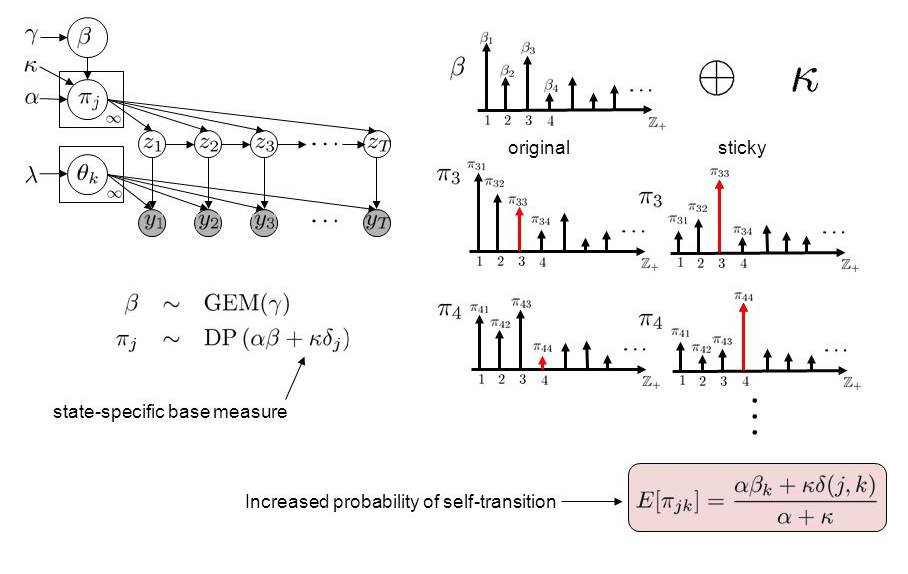
\includegraphics[width=\textwidth]{img/sticky_hdp-hmm.png}

  See also the HDP-HSMM (Johnson, 2013): rules out self-transitions, 
  and models durations separately
  \end{center}
\end{frame}

% ---------------------------------------------------
\begin{frame}
  \frametitle{Local Transitions: The HDP-HMM-LT}
  \begin{itemize}[<+->]
  \item Generalize preference for self-transitions to ``local'' transitions: HDP-HMM-LT.
  \item Latent states located in a space 
    with a symmetric similarity kernel, $\phi$:
    \begin{align}
      0 \leq \phi(\ell_j, \ell_{j'}) = \phi(\ell_{j'}, \ell_j) \leq \phi(\ell_j, \ell_j) \equiv 1
    \end{align}
  \item $P(j \to j')$ from HDP prior is rescaled by $\phi_{jj'}$.
  \end{itemize}
\end{frame}

% ---------------------------------------------------
\begin{frame}
  \frametitle{The HDP-HMM-LT}
  \begin{exampleblock}{\small

      {\bf Definition: HDP-HMM-LT}

\vspace{0.2in}
    Assume we have a sequence of location pairs $\{(\theta_j, \ell_j)\}_{j=1}^\infty$ from some
    distribution, and a similarity kernel $\phi$.  We define
    \begin{align}
      \beta &\sim \mathsf{Stick}(\gamma) \\
      \tilde{\pi}_j &\sim \mathsf{DP}(\alpha\bbeta) \\
      a_{jj'} &= \tilde{\pi}_{jj'} \phi_{jj'} \\
      z_t \given z_{t-1} &\sim \sum_{j'} \frac{a_{z_{t-1}j'}}{\sum_{j''}
        a_{z_{t-1}j''}} \delta_{j'} \\
      y_t \given z_t &\sim F(\theta_{z_t})
    \end{align}
  }
  \end{exampleblock}
  The normalization term is finite and positive since it
  is bounded above by $\sum_{j'} \tilde{\pi}_{jj'} = 1$, and below by $\tilde{\pi}_{jj'}$.
\end{frame}

\begin{frame}
  \frametitle{Normalized Gamma Process Representation}
  The DP can also be obtained by normalizing a {\it Gamma Process}:

\begin{exampleblock}{\small
  A {\bf Gamma Process} is a Poisson Process on $\mathbb{R}^{+} \times
  \Theta$ with L\'evy intensity measure
  \begin{equation}
    \label{eq:8}
    \nu(d\pi, d\theta) = \alpha \pi^{-1} e^{-\pi} d\pi G_0(d\theta)
  \end{equation}

  Consider a random collection of point masses $\{\theta_j\}$
  on $\Theta$, with respective random masses $\{\pi_j\}$ as points
  $(\pi_j,\theta_j) \in \mathbb{R}^+ \times \Theta$.  The number $n(A)$
  of such points in a region $A \subset \mathbb{R}^+ \times \Theta$ is
  distributed
  \begin{equation}
    \label{eq:9}
    n(A) \sim \Pois{\int_A \nu(d\pi, d\theta)}
  \end{equation}
}
\end{exampleblock}

  The normalized set of atoms form a probability measure on $\Theta$.
  This normalized measure is distributed $\mathrm{DP}(\alpha G_0)$.
\end{frame}
% ---------------------------------------------------
\begin{frame}
  \frametitle{A Gamma Process representation}
  By the Gamma Process representation of the DP, we obtain the same
  model by drawing 
  \begin{align*}
    \beta &\sim \mathsf{Stick(\gamma)} \\
    \{\pi_{jj'}\}_{j} &\stackrel{i.i.d.}{\sim} \mathsf{Gamma}(\alpha
      \beta_{j'},1) \qquad j' \geq 1
  \end{align*}
  and setting
\begin{equation*}
    \label{eq:14}
    \tilde{\pi}_{jj'} = \frac{\pi_{jj'}}{\sum_{j''} \pi_{jj''}}
  \end{equation*}
\end{frame}
% ---------------------------------------------------
\begin{frame}
  \frametitle{A Gamma Process representation}
  Combining the two normalizations yields
  \begin{exampleblock}{\small
      {\bf HDP-HMM-LT (Gamma Process Representation)}

    \begin{align*}
      \beta &\sim \mathsf{Stick}(\gamma) \\
      \pi_{jj'} &\sim \mathsf{Gamma}(\alpha\beta_{j'},1) \\
      a_{jj'} &= \pi_{jj'}\phi_{jj'} \\
      z_t \given z_{t-1} &\sim \sum_{j'} \frac{a_{z_{t-1}j'}}{\sum_{j''}
        a_{z_{t-1}j''}} \delta_{j'} \\
      y_t \given z_t &\sim F(\theta_{z_t})
    \end{align*}
}
  \end{exampleblock}
\end{frame}
% ---------------------------------------------------
\begin{frame}
  \frametitle{Loss of Conjugacy for $\bpi$}
  However the likelihood for $\pi_j$ contains a random normalization term, which
  renders all $\pi_j$ conditionally dependent
  \begin{equation}
    \label{eq:17}
    p(\bz \given \pi, \phi) = \prod_{j} \left(\sum_{j''}
      \pi_{jj''}\phi_{jj''}\right)^{-n_{j\cdot}} \prod_{j'} (\pi_{jj'}\phi_{jj'})^{n_{jj'}}
  \end{equation}
  $n_{jj'}:$ \# of transitions from j to $j'$ \\
  $n_{j\cdot}:$ total visits to $j$
  \pause
\vspace{0.2in}

  We can simplify with an ``augmented data'' representation.
\end{frame}
%---------------------------------------------------
\begin{frame}
  \frametitle{The Markov Process With Failed Jumps Representation}
\begin{exampleblock}{\small
    {\bf Lemma}
    Let $(z_t, u'_{t})_{t=1}^T$ be a pure jump Markov process with 
    rate matrix $(a_{jj'})$, $z_t$ the state after the $t$th jump,
    $u'_t$ the time between jump $t-1$ and $t$.  
    
\vspace{0.2in}
    Given $z_{t-1} = j$,
    \begin{enumerate}[(a)]
    \item $u'_{t} \sim \mathsf{Exponential}(\sum_{j'} a_{jj'})$
    \item $P(z_{t} = j') \propto a_{jj'}$
    \item $u'_{t}$ and $z_{t}$ are independent
    \end{enumerate}
  }
  \end{exampleblock}

  Hence, in $n_{k\cdot}$ visits to state $k$, the process spends
  \begin{equation}
    \label{eq:18}
    u_j \sim \mathsf{Gamma}(n_{j\cdot},\sum_{j'}a_{jj'})
  \end{equation}
  time there.
\end{frame}

% ---------------------------------------------------
\begin{frame}
  \frametitle{Introducing failed jumps}
  \begin{exampleblock}{\small 
      {\bf Lemma} Suppose also that while in state $j$, unsuccessful attempts to jump
  to state $j'$ are made at rate $\pi_{jj'} - a_{jj'} = \pi_{jj'}(1 -
  \phi_{jj'})$.  The total number of these is
  \begin{equation}
    \label{eq:19}
    q_{jj'} \sim \mathsf{Poisson}(\pi_{jj'}(1 - \phi_{jj'}) u_j)
  \end{equation}
  }
\end{exampleblock}
\end{frame}
%---------------------------------------------------
\begin{frame}
  \frametitle{Augmented Likelihood for $\pi$}
  Augmenting the data with $u$ and $Q$, the likelihood for $\pi$ becomes
  \begin{align*}
    \label{eq:20}
    \mathcal{L}(\pi \given z, u, Q; \phi) &\propto 
    \prod_{j}\prod_{j'}
    \pi_{jj'}^{n_{jj'} + q_{jj'}} e^{-u_j\pi_{jj'}}
  \end{align*}
  which is conjugate to the Gamma prior.
\end{frame}

%---------------------------------------------------
\subsection{Posterior Inference}
\begin{frame}
  \frametitle{Gibbs Sampling}
  % Cannot deal with full posterior over all parameters
  % analytically, but, after data augmentation, can iteratively sample (1) (hyper)parameters, 
  % and (2) latent state sequence and
  % augmented data, fixing the other at each iteration.
  \begin{itemize}[<+->]
  \item Conditioned on $A$ and the observations, sample the
    state sequence $z$ jointly with a ``message passing'' algorithm.
  \item Sample augmented data from Exponential and Poisson distributions.
  \item Sample $\bpi$ and hyperparameters ($\bbeta$,
    $\alpha$, and $\gamma$) using the factorization
    \begin{equation}
      \label{eq:22}
      p(\gamma, \alpha, \bbeta, \bpi \given \mathcal{D}) = p(\gamma
      \given \mathcal{D}) p(\alpha \given \mathcal{D}) p(\bbeta \given
      \gamma, \mathcal{D}) p(\bpi \given \bbeta, \alpha, \mathcal{D})
    \end{equation}
    where $\mathcal{D}$ is the augmented ``data''.
  \item (We require some additional data augmentation to get the
    marginal distributions for $\gamma$, $\alpha$ and $\beta$.)
  \end{itemize}
\end{frame}

\section{Experiments}
\label{sec:experiments}

\begin{frame}{Cocktail Party Data}
\vspace{-0.3in}
  \begin{center}
    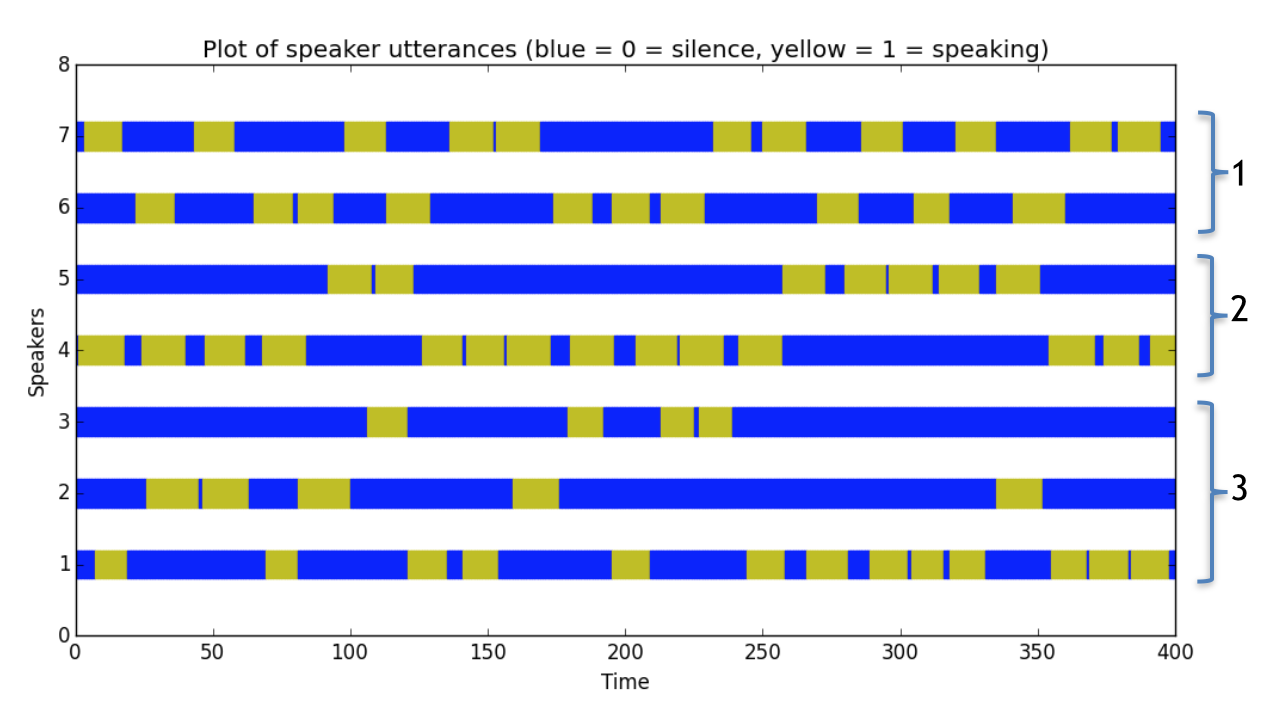
\includegraphics[width=\textwidth]{img/cocktail-with-groups.png}
  \end{center}
\end{frame}

\begin{frame}{Similarity and Emission Model}
\begin{itemize}
\item Latent states: binary vectors, $\{\theta_j\}$
\item $F$: Normal linear model
\item $\phi_{jj'} = \exp(-\lambda \left\Vert\theta_j -
\theta_{j'}\right\Vert_{L_1})$
\end{itemize}
\end{frame}

\begin{frame}{Recovery of Binary States ($F_1$ measure)}
\vspace{-0.4in}
    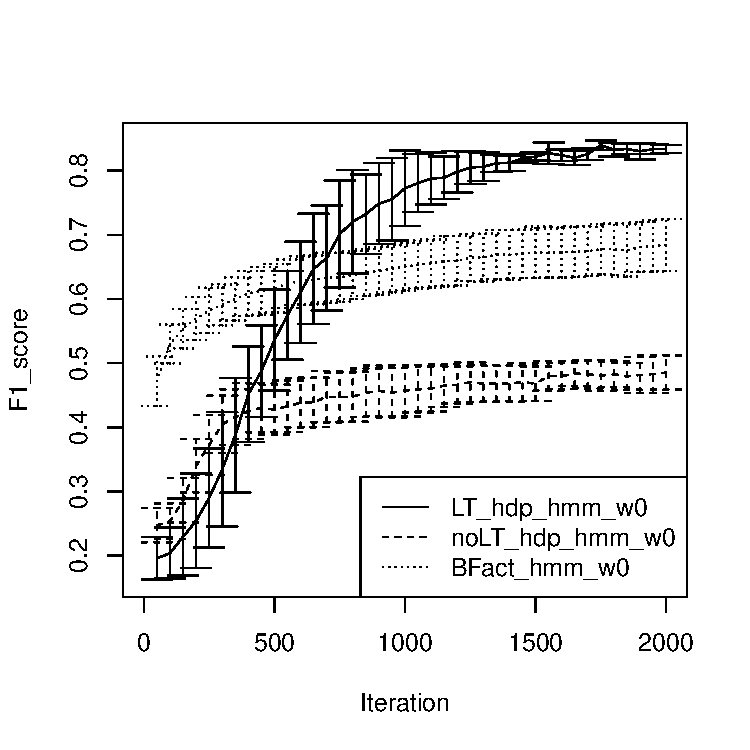
\includegraphics[width=0.9\textwidth]{img/cocktail/F1_score.pdf}
    Error bars: 99\% CI of the mean per iteration, based on 10 Gibbs runs
\end{frame}
\begin{frame}{Similarity Parameter}
\vspace{-0.4in}
    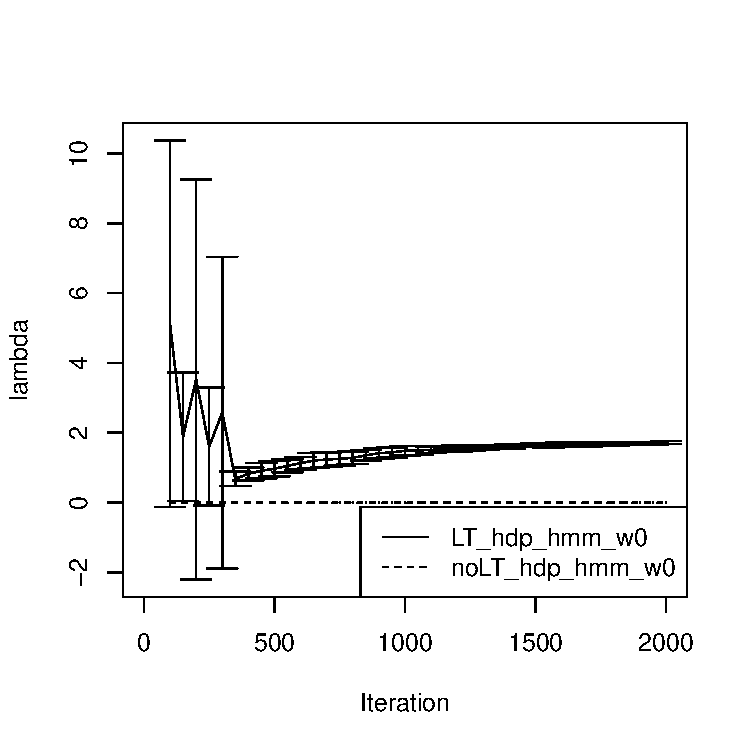
\includegraphics[width=0.9\textwidth]{img/cocktail/lambda.pdf}
    Error bars: 99\% CI of the mean per iteration, based on 10 Gibbs runs
\end{frame}
\begin{frame}{Number of States Found}
\vspace{-0.4in}
    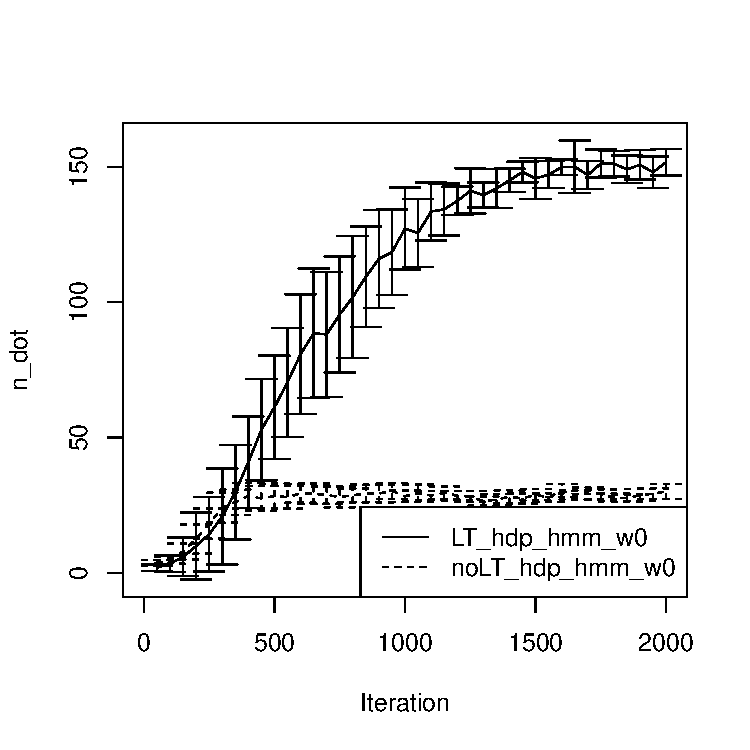
\includegraphics[width=0.9\textwidth]{img/cocktail/n_dot.pdf}
    Error bars: 99\% CI of the mean per iteration, based on 10 Gibbs runs
\end{frame}

\begin{frame}{Inferred Speaker Sequence}
  \begin{center}
    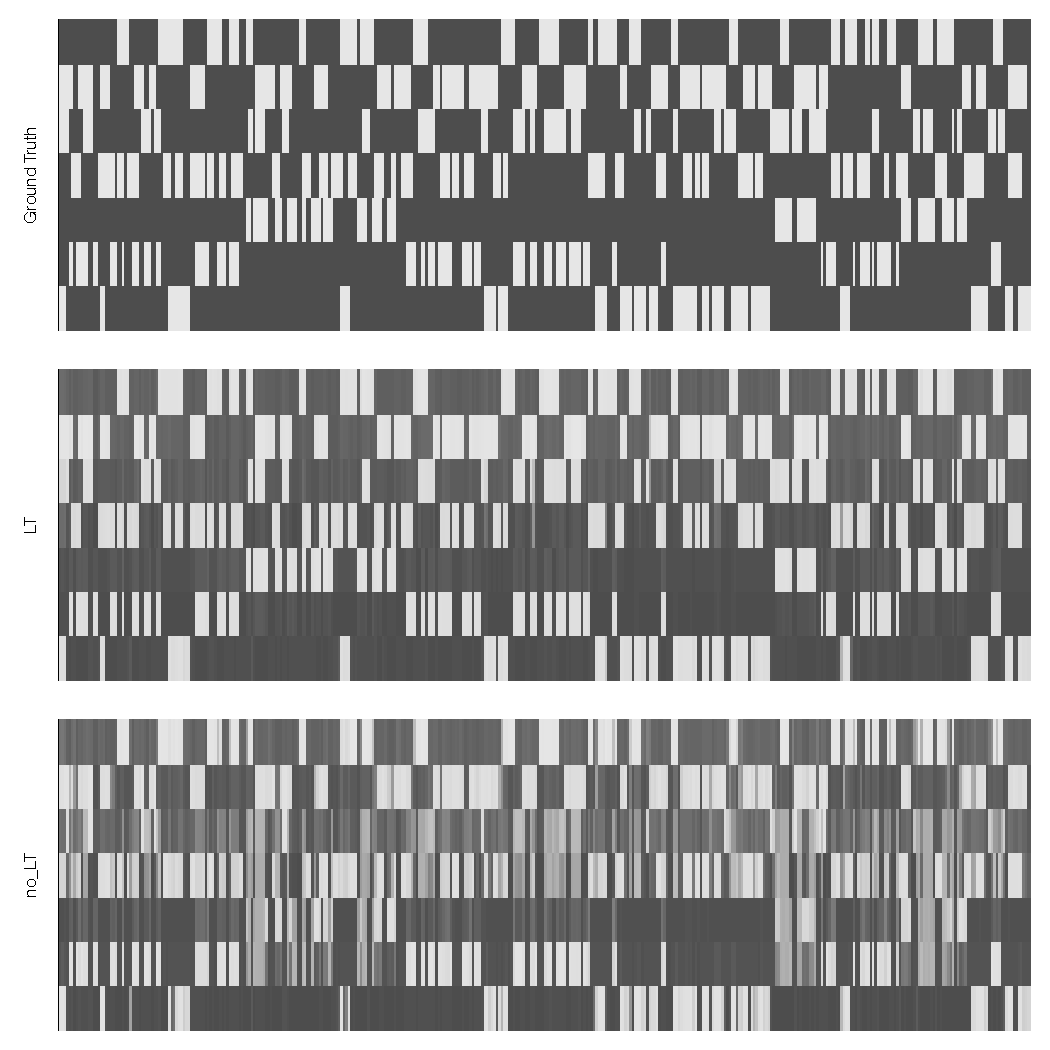
\includegraphics[width=\textwidth,height=0.75\textwidth]{img/hdp-hmm-lt_grid.pdf}
  \end{center}
\end{frame}

\subsection{Data With Block Diagonal Transitions}
\begin{frame}{(Near) Block Diagonal Transition Matrix}
\label{sec:block-diag-trans}
\begin{minipage}{0.45\textwidth}
\begin{center}
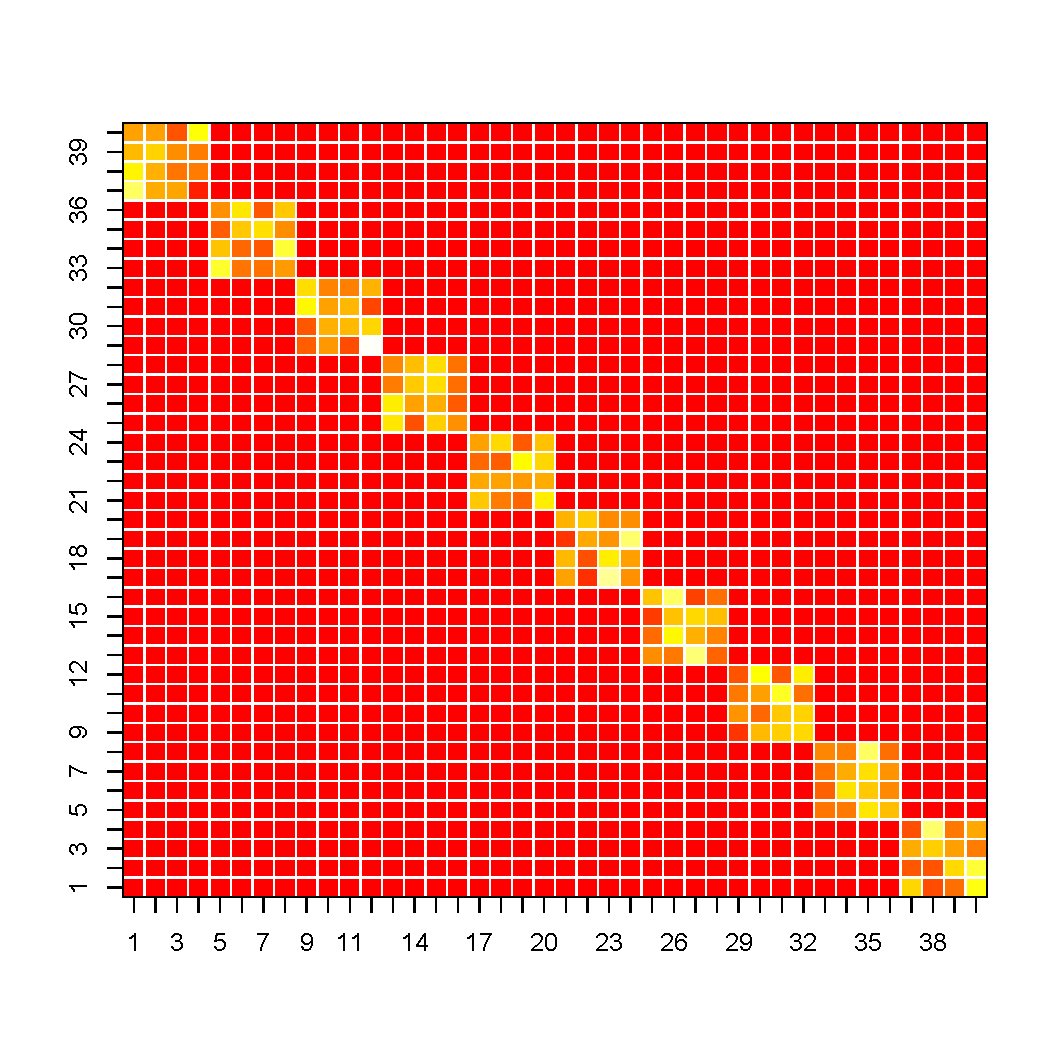
\includegraphics[width=\textwidth]{img/block_diag/A_gt_10x4}
\end{center}
\end{minipage}
\hspace{0.1in}
\begin{minipage}{0.45\textwidth}
\begin{center}
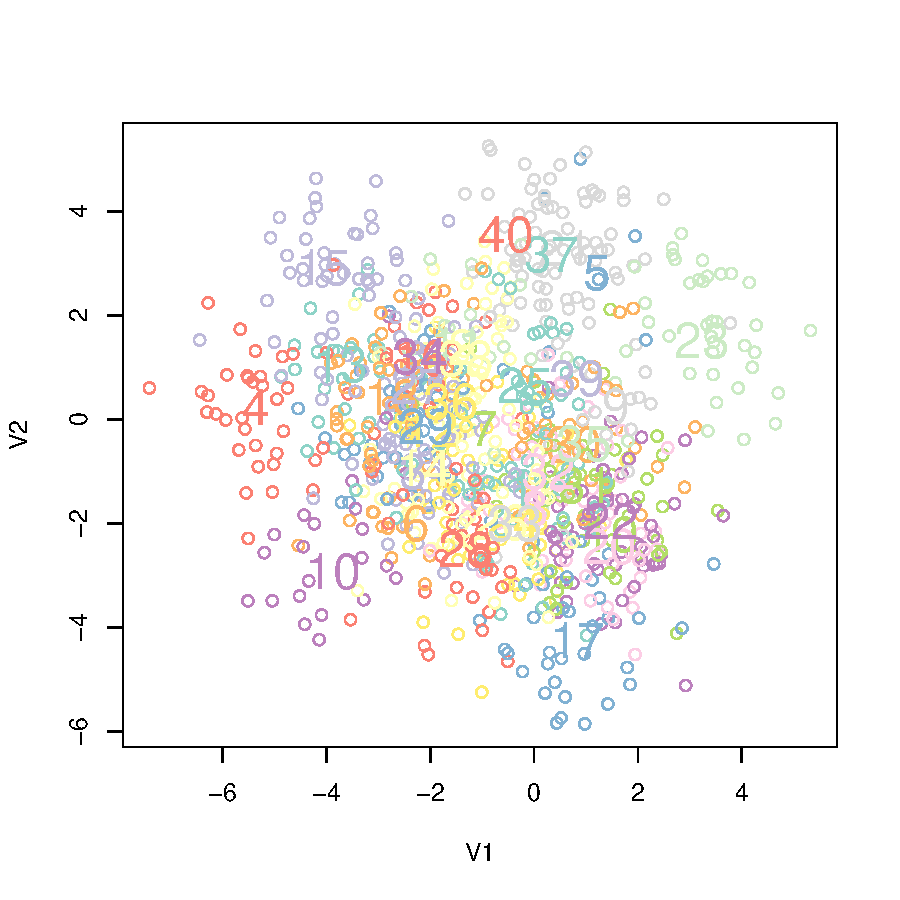
\includegraphics[width=\textwidth]{img/block_diag/10x4_gty}
\end{center}
\end{minipage}
Many more transitions ``within groups''.\\
Unlike previous experiment, similarity via $\phi$ and similarity in
emissions are decoupled.
\end{frame}
\begin{frame}{Block Diagonal Experiment}
  \begin{itemize}[<+->]
  \item Data: 95\% within group transitions
  \item Emission model is Normal: $\theta = (\mu, \Sigma)$
  \item Similarity is Gaussian kernel:
    \begin{equation*}
      \phi(\eta_j, \eta_{j'}) = \exp(-\lambda \left \Vert \eta_{j} -
          \eta_{j'} \right \Vert_{L_2}^2)
    \end{equation*}
  \item $\eta$ locations in an abstract latent space; ``likelihood''
    in terms of Bernoulli process of successful and failed transitions
    \begin{equation*}
      p(z, Q \given \eta) = \prod_{j}\prod_{j'} \phi_{jj'}^{n_{jj'}}
      (1 - \phi_{jj'})^{q_{jj'}}
    \end{equation*}
  \item Infer $\eta$ separately from $\theta$, using a Hamiltonian
    Monte Carlo (HMC) step (Duane and Pendleton, 1987)
  \end{itemize}
\end{frame}

\begin{frame}{Results: LT vs no LT}
\begin{figure}
\begin{minipage}{0.45\textwidth}
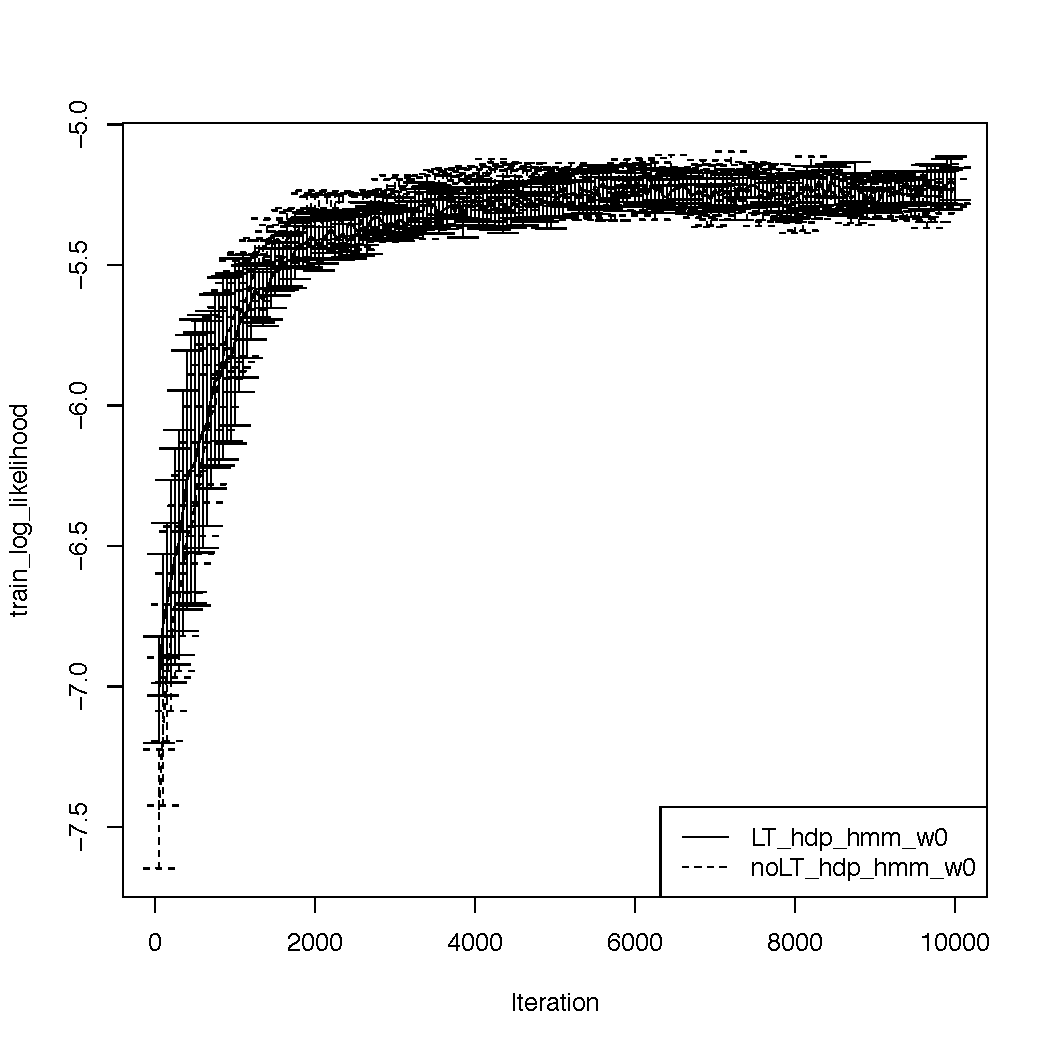
\includegraphics[width=\textwidth]{img/block_diag/train_log_likelihood}
\end{minipage}
\hspace{0.1in}
\begin{minipage}{0.45\textwidth}
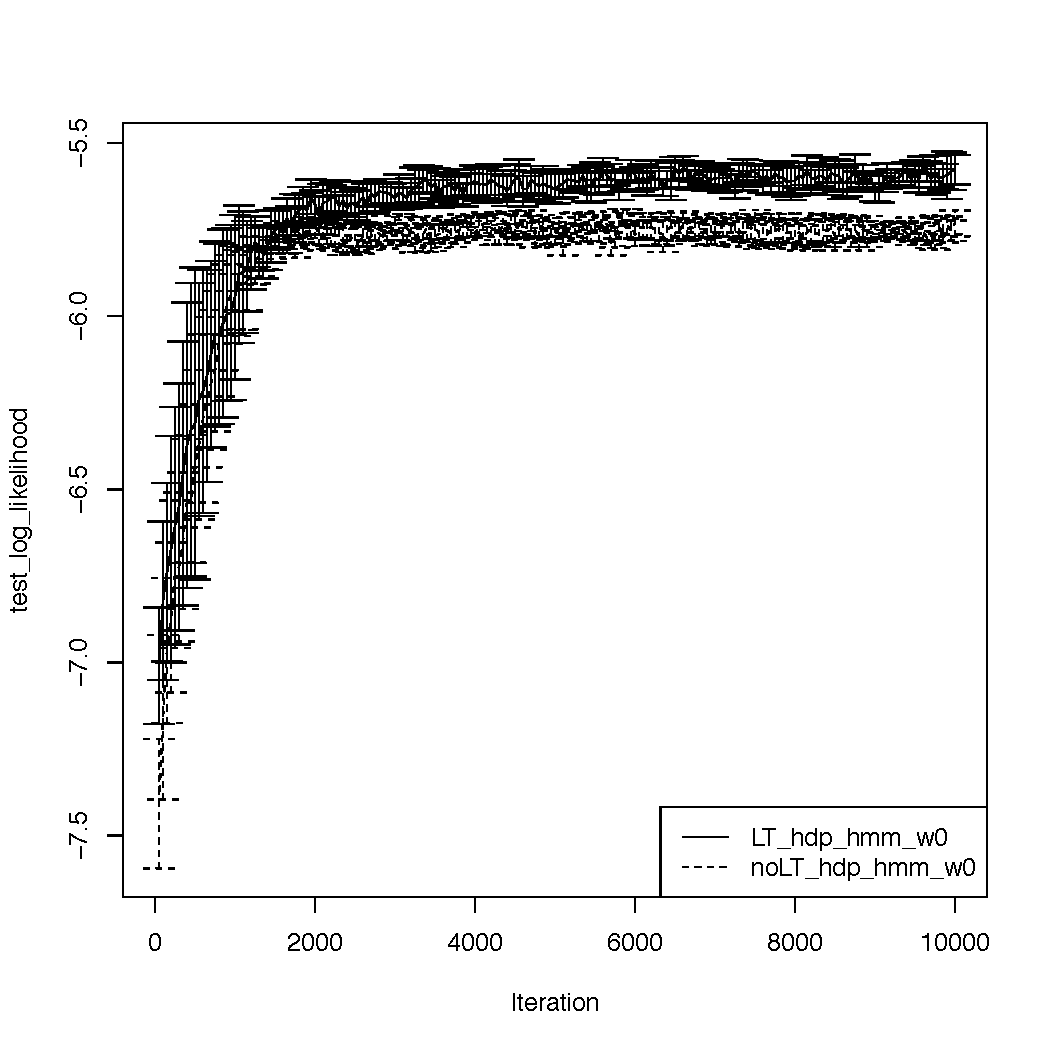
\includegraphics[width=\textwidth]{img/block_diag/test_log_likelihood}
\end{minipage}
\caption{Left: Log likelihood on the training set by Gibbs iteration
  (marginalizing out state sequence) for LT and no LT (HDP-HMM)
  models.  Right: Log likelihood on a held out test set.}
\end{figure}
\end{frame}

\begin{frame}{Inferred Transition Matrices}
\begin{figure}
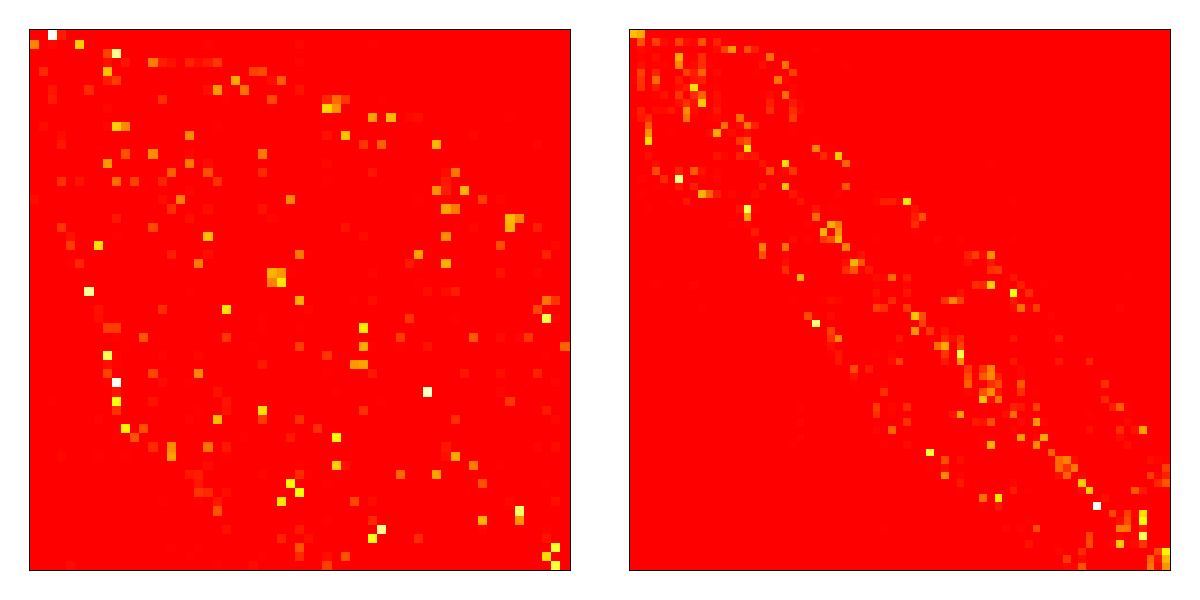
\includegraphics[width=\textwidth]{img/block_diag/A01}
\caption{Left: Inferred transition matrix using the noLT (HDP-HMM)
  model. Right: Inferred transition matrix using the LT model.  State
  permutation found using Reverse Cuthill-McKee algorithm.}
\end{figure}
\end{frame}

\begin{frame}{Inferred Transition Matrices}
\begin{figure}
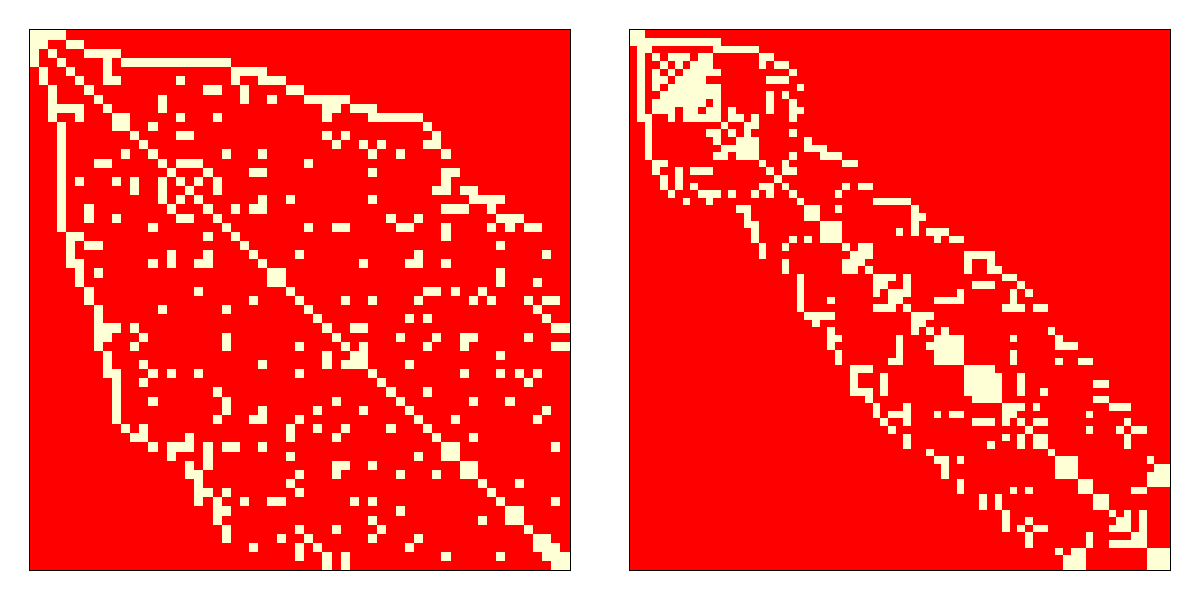
\includegraphics[width=\textwidth]{img/block_diag/A01-binary}
\caption{Left: Inferred transition matrix using the noLT (HDP-HMM)
  model. Right: Inferred transition matrix using the LT model.  State
  permutation found using Reverse Cuthill-McKee algorithm.}
\end{figure}
\end{frame}

\begin{frame}{Ongoing: Discovering Chord Classes in Music}
  \begin{figure}
    \centering
    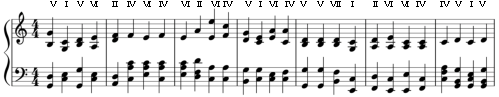
\includegraphics[width=\textwidth]{img/chords_annotated.pdf}
    \caption{Transcription of a four-voice chorale, annotated with chord classes}
  \end{figure}
  \begin{itemize}
  \item Encode each unique chord as an integer
  \item Infer latent states w/ LT vs no-LT, using a categorical
    emission model
  \end{itemize}
\end{frame}

\begin{frame}{Results: Emission Distributions}
  \begin{figure}
    \centering
    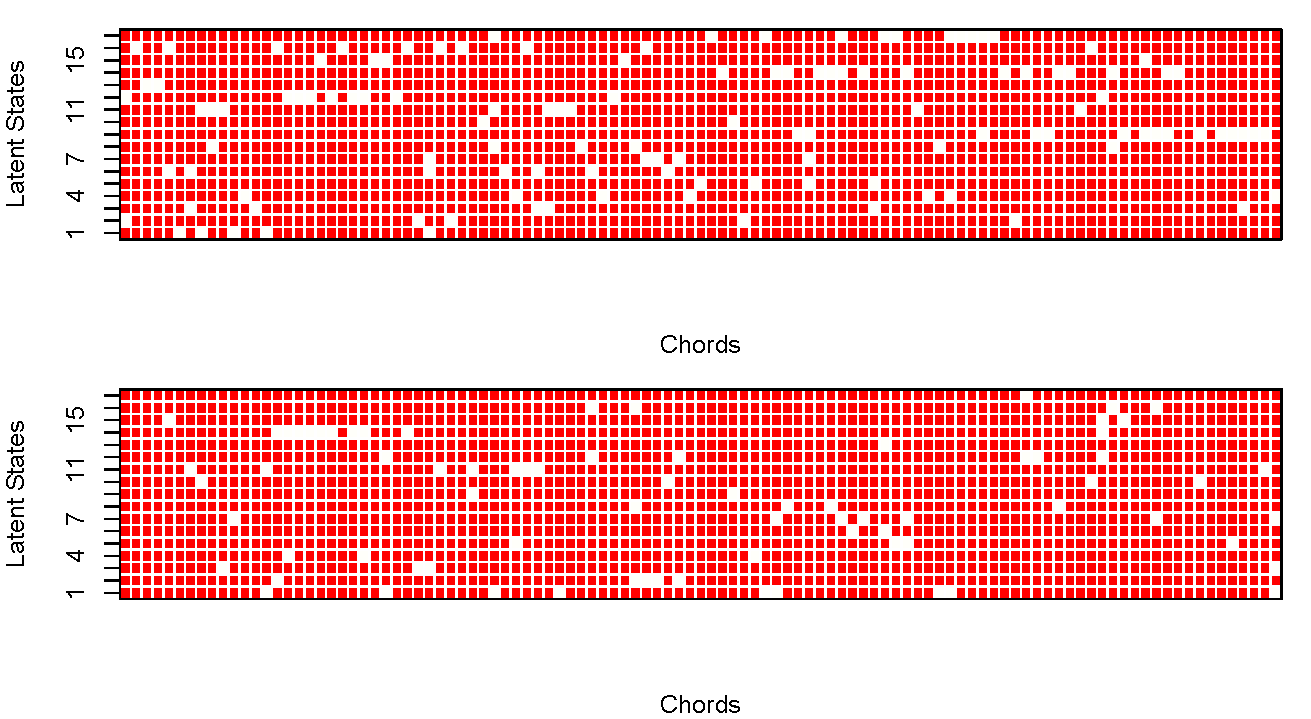
\includegraphics[width = \textwidth]{img/chord_emissions.pdf}
    \caption{Emission distributions for states used (normalized by
      overall chord frequency, and thresholded).  Top: no LT, Bottom: LT}
  \end{figure}
\end{frame}

% ---------------------------------------------------
\begin{frame}
  \begin{exampleblock}{\small
      {\bf Summary of Contributions}
\vspace{0.2in}

    \begin{itemize}
      \item A new model, the HDP-HMM-LT, in which there is a
        notion of geometry of the transition state space, such that
        transitions are more likely between nearby states.
      \item Formulation of HDP-HMM-LT as the marginalization of
        the ``Markov Process With Failed Jumps''.
      \item A straightforward Gibbs sampler after data augmentation
      \item Better generalization than existing models on data w/
        nearby state changes
    \end{itemize}
}
\end{exampleblock}
\end{frame}

\section{Future Work}
\label{sec:future-work}

\begin{frame}{Ongoing: Power Disaggregation}
\begin{minipage}{0.45\textwidth}
  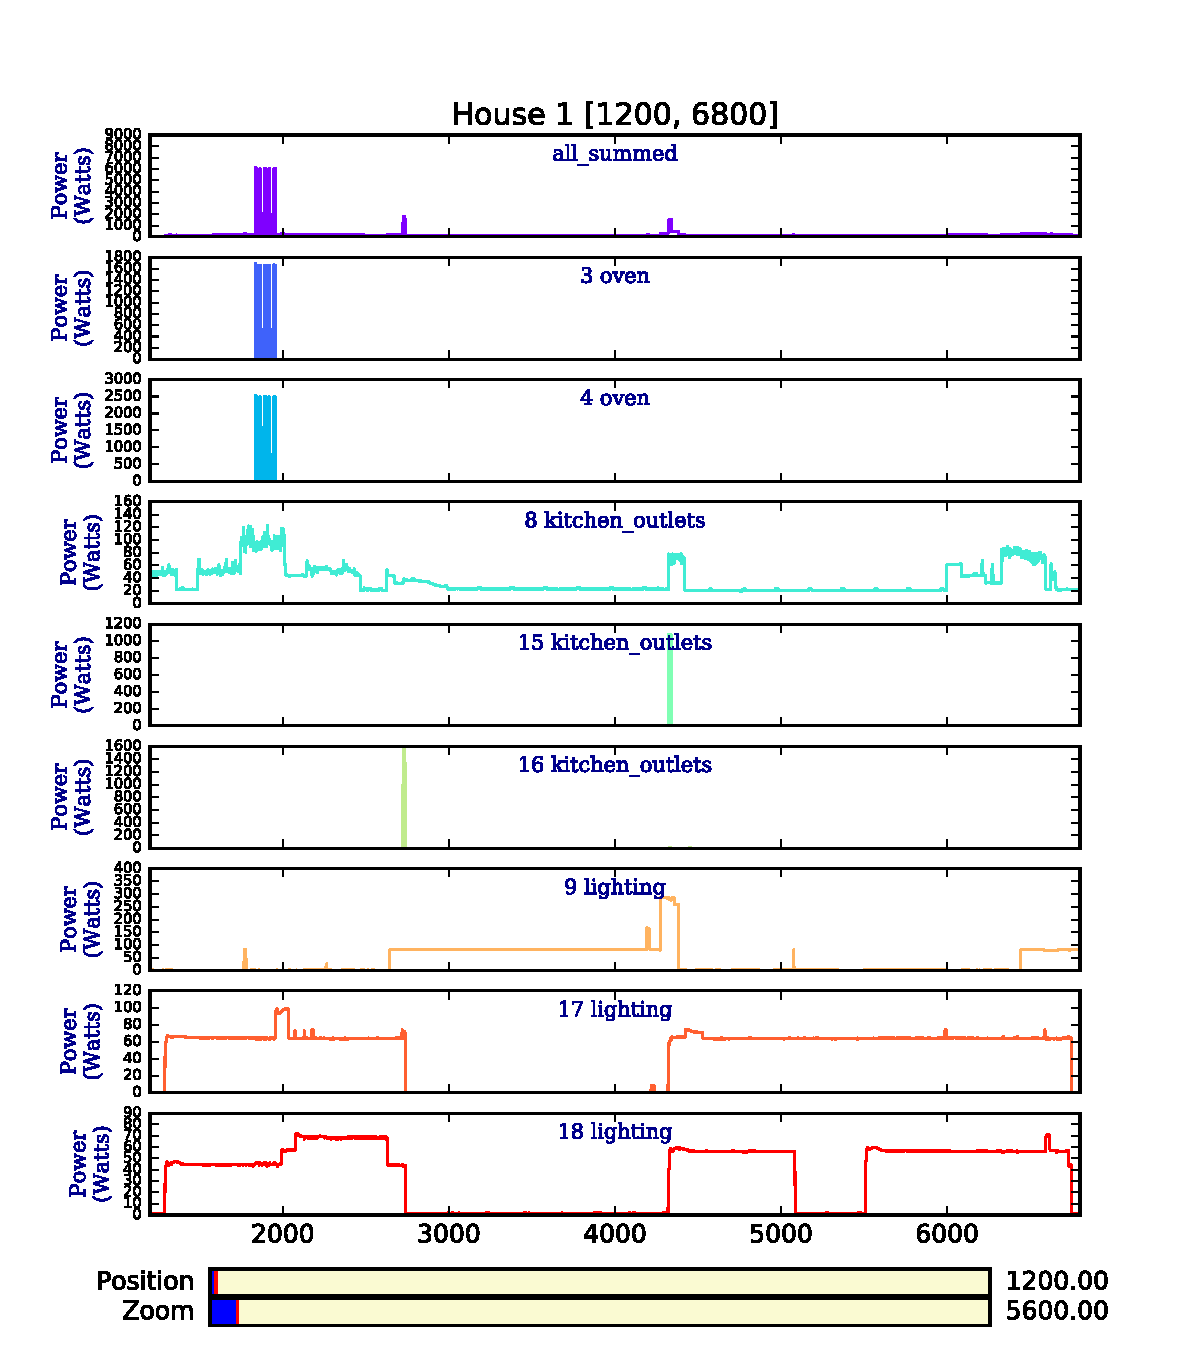
\includegraphics[width=\textwidth]{img/redd_data.pdf}
\end{minipage}
\hspace{0.1in}
\begin{minipage}{0.45\textwidth}
  \begin{itemize}
  \item Data: Time series of total power consumptioo 
  \item Latent state: How much power is each channel using at each
    time
  \item Different appliances have different discrete set of ``modes''
  \end{itemize}
\end{minipage}
\end{frame}

\begin{frame}{Future: Discovering Biological Context}
  \begin{center}
    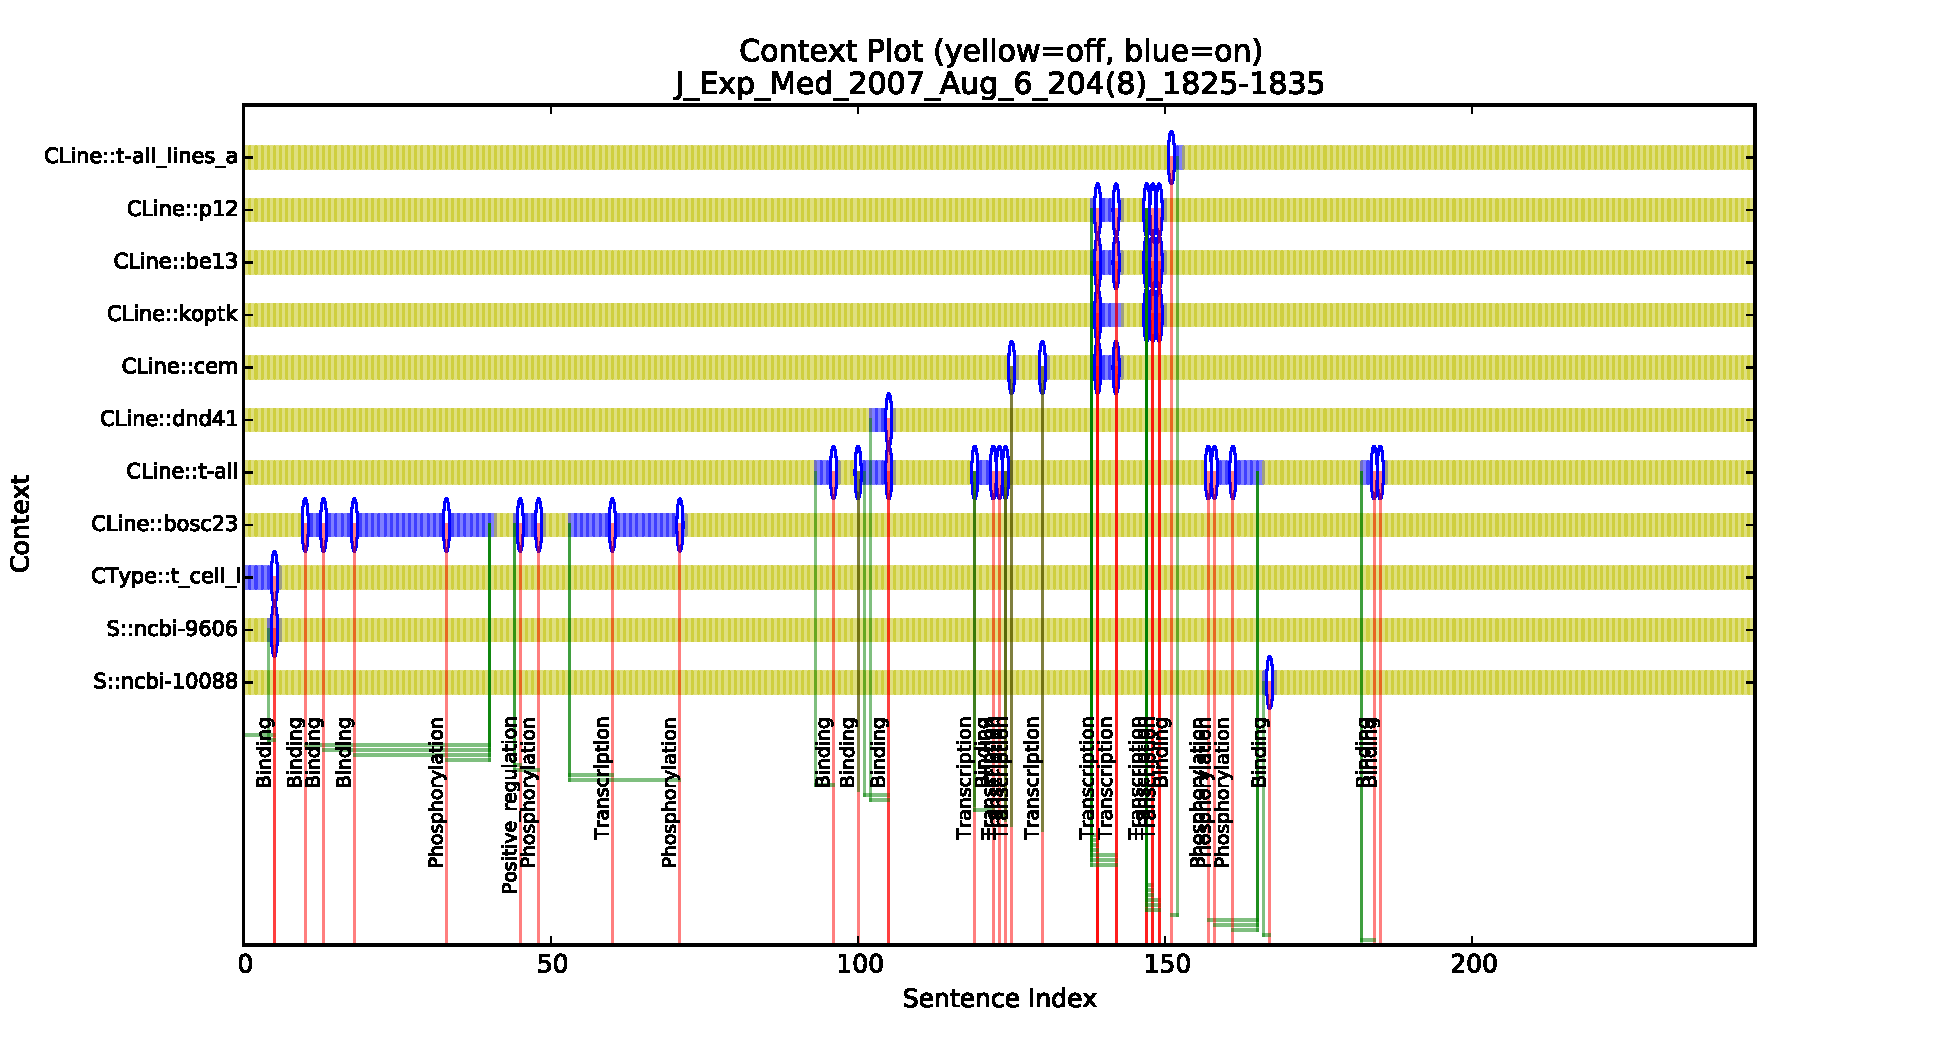
\includegraphics[width=\textwidth]{img/bio_contexts.pdf}
  \end{center}
\end{frame}

\begin{frame}{Theoretical Challenges}
  \begin{itemize}[<+->]
  \item Beam sampling
    \begin{itemize}
    \item Now: need to bound the number of states considered
    \item Beam sampling: adaptively considers new states (slice
      sampling)
    \item But, auxiliary representation of $u$ and $Q$ requires
      explicit representation
    \end{itemize}
  \item Adaptive HMC
    \begin{itemize}
    \item In HMC need to hand-tune step size.  Incorporate
      ``adaptive'' methods based on Riemannian manifolds.
    \end{itemize}
  \end{itemize}
\end{frame}

\end{document}

